\chapter{Diseño}
\label{cap:capitulo4}

En este capítulo se describe el trabajo realizado y los experimentos llevados a cabo para validar el desarrollo.\\

El trabajo, como se explicó en el Capítulo 2, se ha dividido en dos fases; primero se realiza una simulación del coche autónomo en una ciudad simplificada, para a continuación, reproducir ese mismo escenario en un entorno real.\\

\section{Entorno simulado}
\label{section:simulation}
Para poder simular el comportamiento deseado en un entorno simulado es necesario disponer de dos elementos; un modelo del coche autónomo y un mundo dinámico con el que el vehículo interactuará, todo ello ejecutado dentro de un simulador, en este caso, como se explicó anteriormente, en \textit{Gazebo}.\\

\subsection{Modelo de la ciudad}
\label{subsection:citymodel}
Existen numerosos mundos diseñados para \textit{Gazebo} disponibles en repositorios de \textit{GitHub}\footnote{\url{https://github.com/chaolmu/gazebo_models_worlds_collection}}\footnote{\url{https://github.com/mlherd/Dataset-of-Gazebo-Worlds-Models-and-Maps}}. En el caso que se plantea, es necesario una ciudad, por lo que partiendo de una ciudad\footnote{\url{https://github.com/chaolmu/gazebo_models_worlds_collection/blob/master/worlds/small_city.world}} de gran tamaño se reduce su tamaño con el objetivo de, posteriormente, poder reproducir ese escenario en el mundo real. En la Figura \ref{fig:cityversus} se observan ambas ciudades.\\

\begin{figure} [h!]
	\begin{center}
		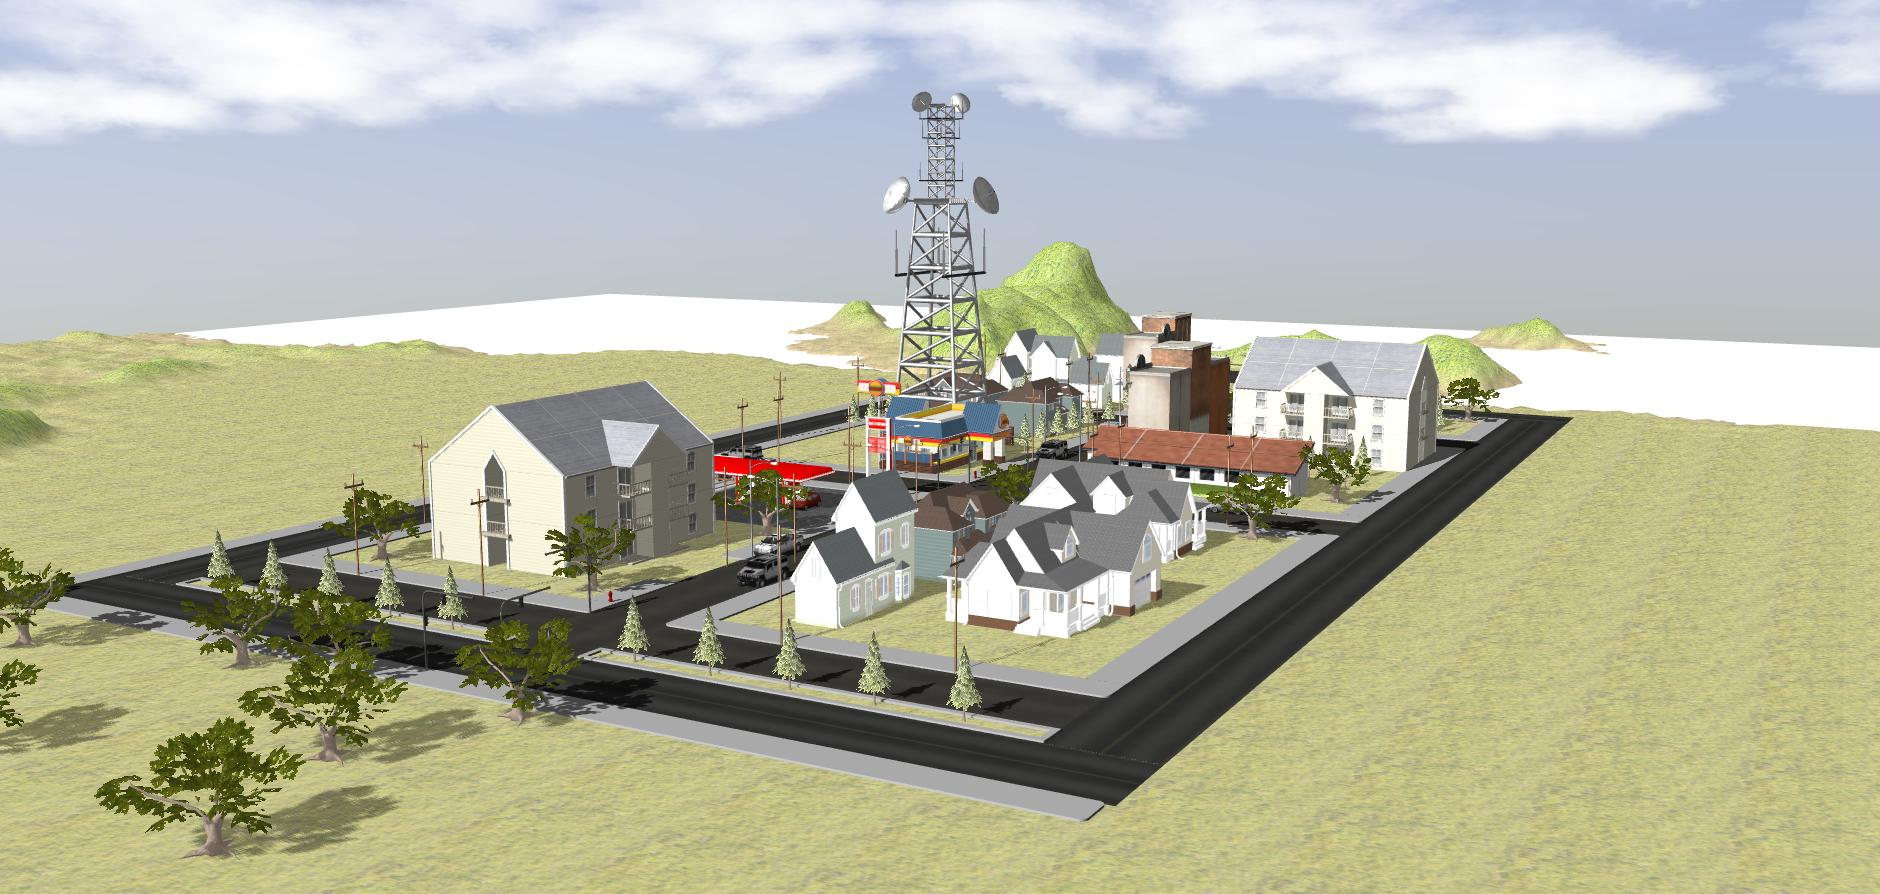
\includegraphics[width=7cm]{figs/city2}\hspace{1cm}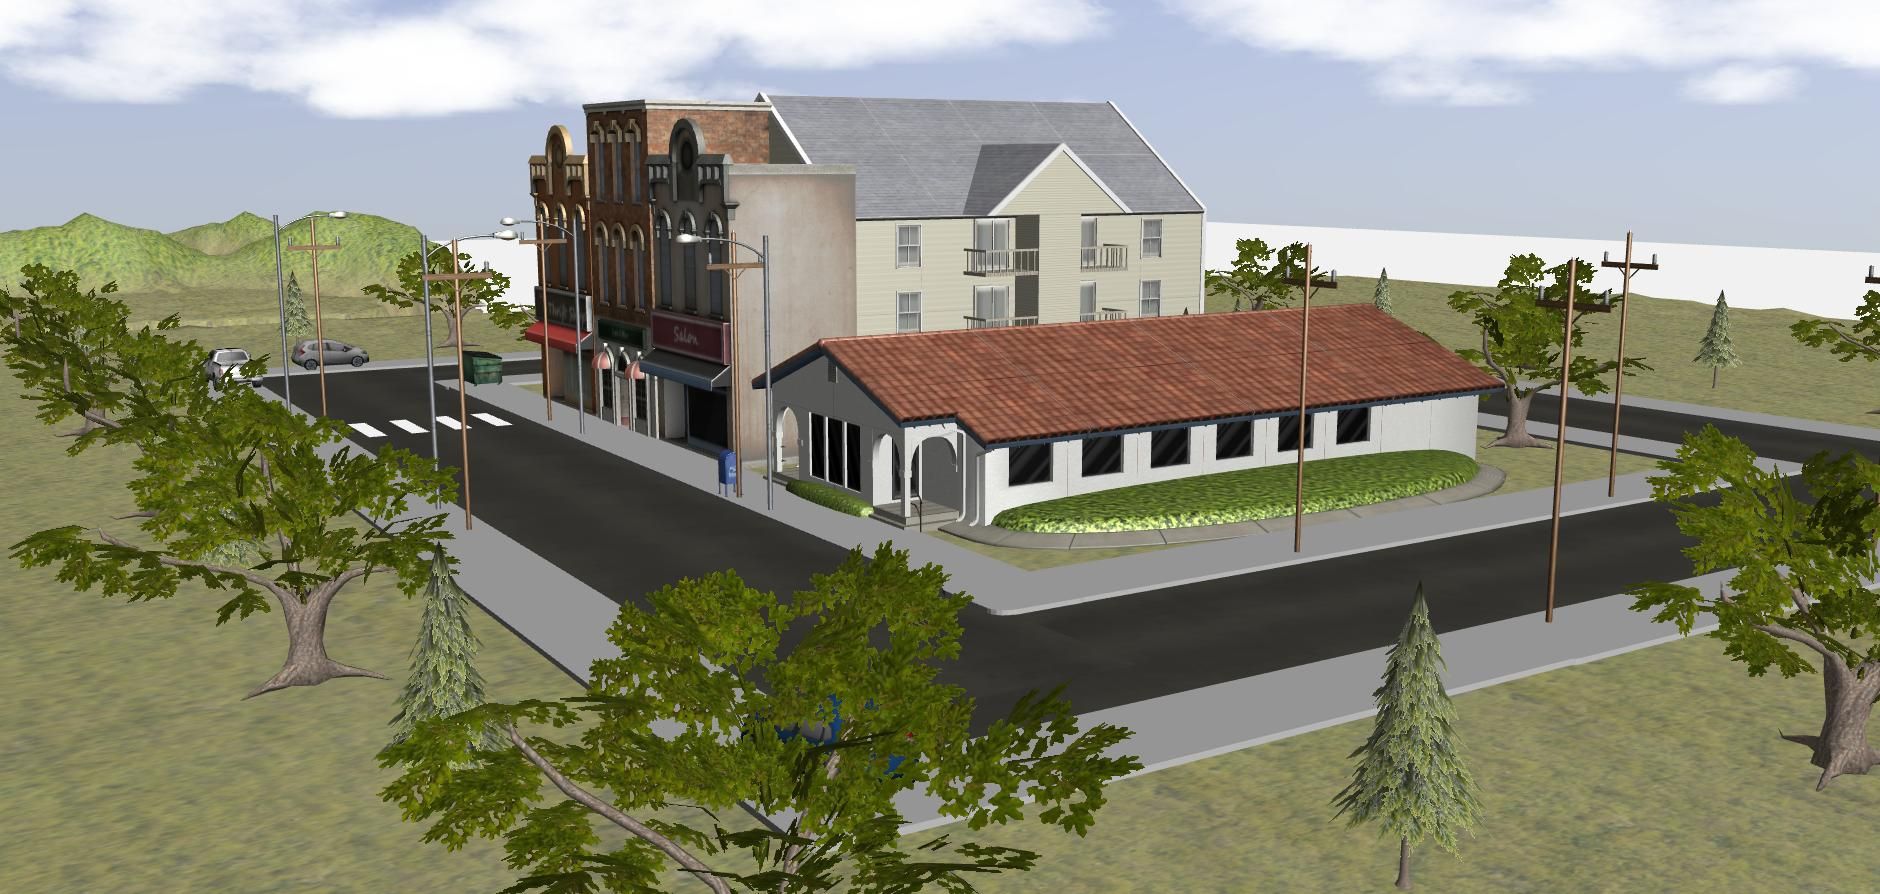
\includegraphics[width=7cm]{figs/smallcity}
	\end{center}
	\caption{Modelo de la ciudad original y la ciudad modificada en \textit{Gazebo}.}
	\label{fig:cityversus}
\end{figure}\

El modelo de esta ciudad es estático, es decir, no contiene elementos dinámicos, por lo que es necesario añadir dos tipos de elementos; un semáforo y un peatón que cruce un paso de peatones. Para ello, es necesario añadir dos \textit{plugins} para \textit{Gazebo}. En primer lugar, y usando un modelo \textit{SDF} que integra el \textit{plugin} de cambio de color en el semáforo\footnote{\url{https://github.com/robustify/gazebo_traffic_light}}. Dicho \textit{plugin} tiene asociado un fichero de configuración en formato \textit{YAML}, Código \ref{cod:trafficlight}, en el que se especifica la secuencia de estados del semáforo y su duración en el tiempo.\\

\begin{code}[h]
	\begin{lstlisting}
		light_sequence:
  - { color: "green", duration: 10, flashing: false }
  - { color: "yellow", duration: 1, flashing: false }
  - { color: "red", duration: 50, flashing: false }
	\end{lstlisting}
	\caption[Definición de estados y duraciones del semáforo.]{Definición de estados y duraciones del semáforo.}
	\label{cod:trafficlight}
\end{code}

El segundo \textit{plugin} proporciona movimiento a un modelo de un humano llamado actor. Está disponible en otro repositorio\footnote{\url{https://github.com/BruceChanJianLe/gazebo-plugin-autonomous-actor}} de \textit{GitHub} y permite que el humano se desplace en el mundo de forma realista. El \textit{plugin} citado también permite configuración para especificar la ruta de puntos o \textit{waypoints} que el peatón ha de seguir, así como, su velocidad o la distancia mínima a la que debe situarse respecto a un obstáculo. Dicha configuración se realiza directamente en el fichero \textit{SDF}, como muestra el Código \ref{cod:pedestrianconfiguration}.\\

\begin{code}[h]
	\begin{lstlisting}
		<actor name="actor">
			[...]
			<plugin name="trajectory" filename="libTrajectoryActorPlugin.so">
					<target>
					2.4028 -6.9143 1.1 1.570796 -0.0 3.141593
				</target>
					<target>
					2.4028 6.6816 1.1 1.570796 -0.0 3.141593
				</target>
					<velocity>0.75</velocity>
					<obstacle_margin>1.5</obstacle_margin>
					<obstacle></obstacle>
				</plugin>
			</actor>
	\end{lstlisting}
	\caption[Configuración de \textit{waypoints}, velocidad y distancia a obstáculos del peatón.]{Configuración de \textit{waypoints}, velocidad y distancia a obstáculos del
		peatón.}
	\label{cod:pedestrianconfiguration}
\end{code}

Ambos modelos se sitúan en una paso de peatones, creado a partir de láminas blancas, produciendo el resultado de la Figura \ref{fig:trafficlightpedestrian}.\\

\begin{figure} [h!]
	\begin{center}
		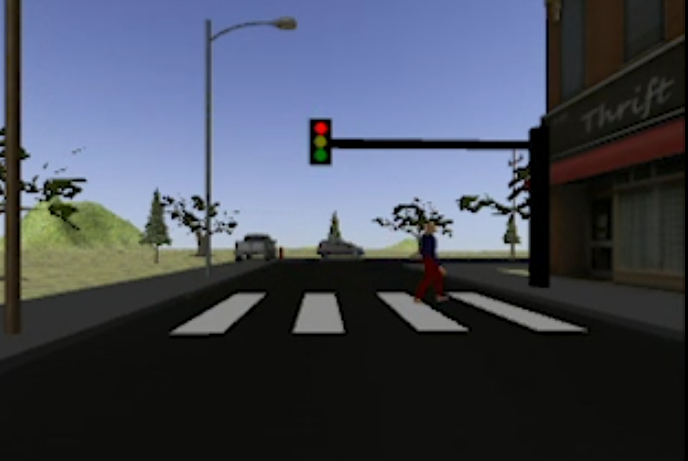
\includegraphics[width=8cm]{figs/trafficlightpedestrian}
	\end{center}
	\caption{Semáforo y peatón usando \textit{plugins} para \textit{Gazebo}.}
	\label{fig:trafficlightpedestrian}
\end{figure}\

\subsection{Modelo del coche autónomo}
\label{subsection:vehiclemodel}
El primer paso para desarrollar un modelo es diseñar las piezas a utilizar, para ello, como se explicó en el Capítulo 2, se utilizará \textit{FreeCAD}. El segundo paso es ensamblar el robot con \textit{Blender} utilizando el \textit{add-on} \textit{Phobos} para definir los \textit{links} y \textit{joints} del robot con el objetivo de dotar al robot de movimiento, generando un fichero \textit{URDF}. Por último, es necesario modificar el \textit{URDF} para añadir cámaras y controladores para los motores que serán usados en el simulador \textit{Gazebo}.\\

\subsubsection{Diseño de las piezas en \textit{FreeCAD}}

A través de la herramienta \textit{Sketcher}\footnote{\url{https://wiki.freecadweb.org/Sketcher_Workbench}}, disponible en \textit{FreeCAD}, es posible realizar un diseño de piezas en 2D con restricciones de horizontalidad, verticalidad, igualdad entre rectas, medidas, ángulos etc y después convertir dicha pieza en 3D proporcionando un volumen a la pieza. Utilizando dicha herramienta se diseña el chasis y las ruedas del vehículo tomando las medidas reales, lo que da como resultado el diseño de las piezas en 2D de la Figura \ref{fig:design2Dfreecad}.\\

\begin{figure} [h!]
	\begin{center}
		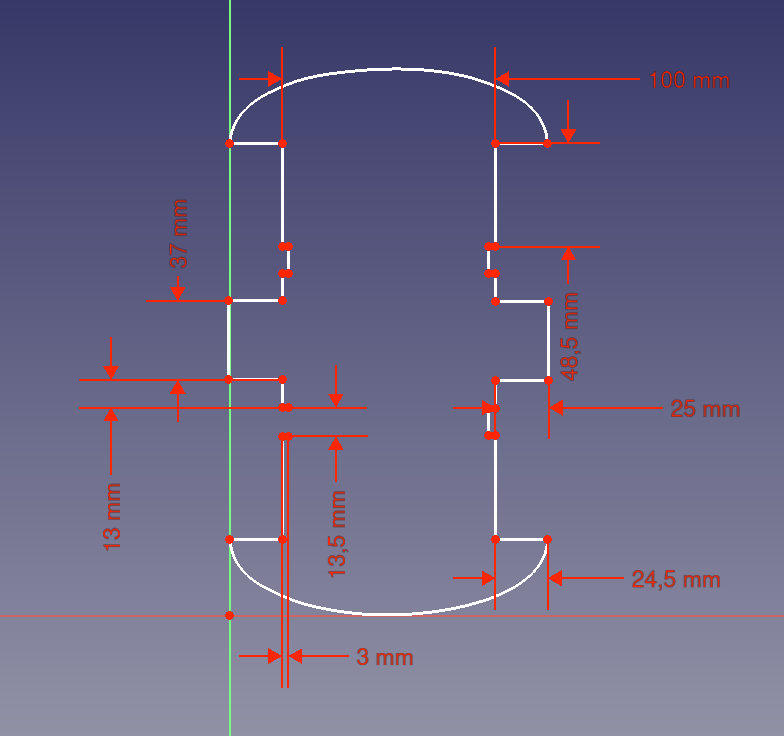
\includegraphics[width=8cm]{figs/sketchFreecad}
	\end{center}
	\caption{Diseño del chasis 2D en \textit{FreeCAD}.}
	\label{fig:design2Dfreecad}
\end{figure}\

A continuación se proporciona un grosor al chasis de 3mm y a las ruedas de xmm, obteniendo el modelo 3D de la Figura \ref{fig:design3Dfreecad}.\\

\begin{figure} [h!]
	\begin{center}
		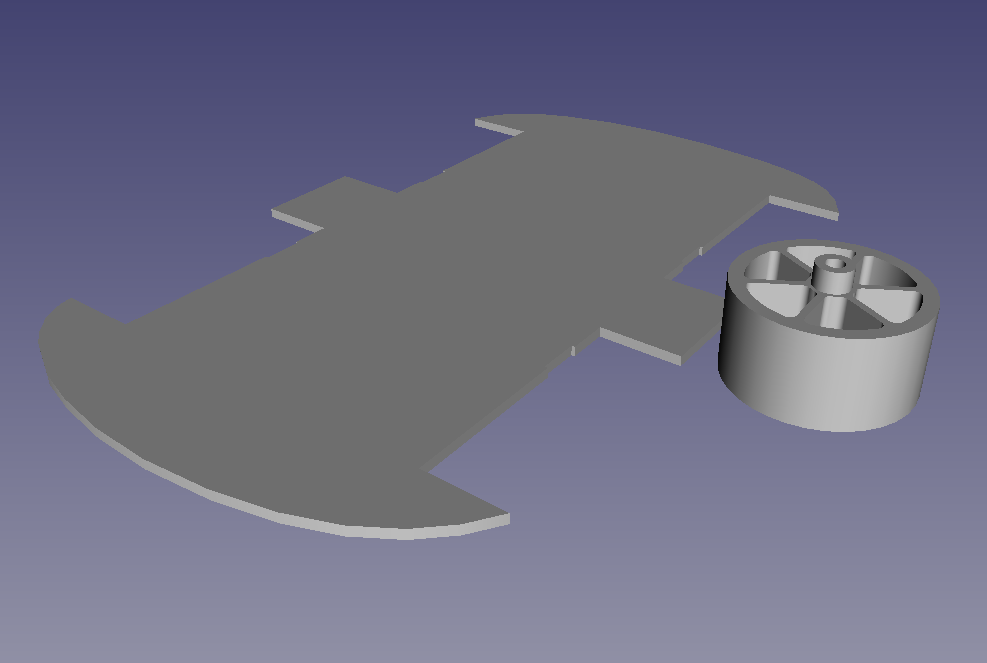
\includegraphics[width=8cm]{figs/freecad}
	\end{center}
	\caption{Diseño de las piezas 3D en \textit{FreeCAD}.}
	\label{fig:design3Dfreecad}
\end{figure}\

El siguiente paso es exportar las piezas diseñadas en formato \textit{STL} para utilizarlas en \textit{Blender}.\\

\subsubsection{Ensamblado del robot en \textit{Blender}}

Una vez importadas las piezas diseñadas en \textit{FreeCAD}, se crean dos unidades del chasis y cuatro ruedas, a continuación se mueven y rotan en el espacio para situarlas correctamente. Con el objetivo de dotar de mayor realismo al modelo, se importan modelos de los motores\footnote{\url{https://grabcad.com/library/tt-motor-1}} y la placa\footnote{\url{https://github.com/57Bravo/jetson_nano_enc}} utilizados. Y se diseñan dos piezas para emular la batería y la cámara del robot. Con todo ello se conforma el modelo estático del robot, Figura \ref{fig:blendermodel}.\\

\begin{figure} [h!]
	\begin{center}
		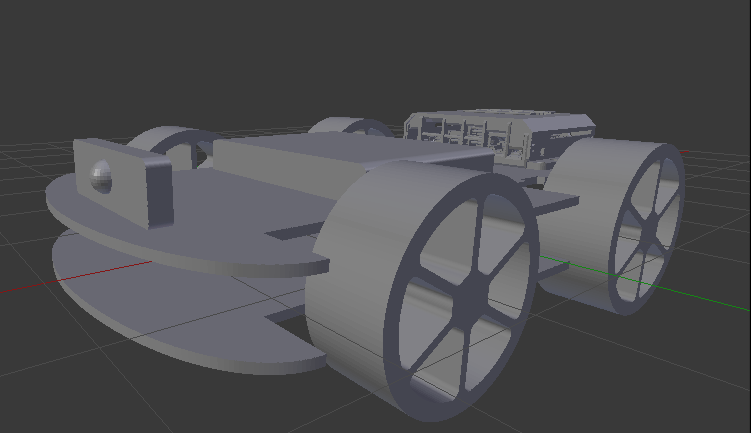
\includegraphics[width=8cm]{figs/blenderModel}
	\end{center}
	\caption{Modelo 3D estático ensamblado en \textit{Blender}.}
	\label{fig:blendermodel}
\end{figure}\

Este modelo es estático, es decir, no es posible simular un movimiento. Para ello es necesario un \textit{add-on} para \textit{Blender} como \textit{Phobos}, que como se explicó anteriormente, permite crear \textit{links} y \textit{joints} y definir una jerarquía entre ellos.\\

En primer lugar, es necesario definir los elementos visuales que compondrán el modelo, en este caso serán todas las piezas del robot, dichas piezas serán del tipo \textit{mesh}, ya que no son objetos primitivos, como cajas o esferas.\\

A continuación, se define un \textit{link} principal que será el cuerpo del robot, de este \textit{link} dependerán las cuatro ruedas del vehículo. Con el objetivo de simular colisiones, se crea un modelo de colisión de cada una de las piezas y un modelo inercial, que estará relacionado con el peso simulado de cada pieza.\\

Por último, se definen los \textit{joints} de cada rueda. A través de está funcionalidad es posible aplicar fuerza o velocidad a las ruedas del robot. Existen diferentes tipos de
\textit{joints} en \textit{Phobos}; \textit{fixed}, \textit{revolute}, \textit{continuous}, \textit{prismatic}, en este caso, son necesarios \textit{joints} de tipo \textit{continuous}, ya que las ruedas realizan un giro sin un límite fijado, y no un movimiento transversal.\\

Una vez definidos todos los elementos del modelo y su jerarquía, en el menú lateral de \textit{Blender} se encontrará el diagrama del modelo, Figura \ref{fig:blenderdiagram}.\\

\begin{figure} [h!]
	\begin{center}
		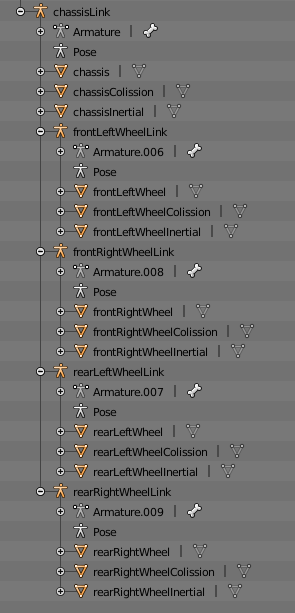
\includegraphics[width=6cm]{figs/phobosDiagram}
	\end{center}
	\caption{Diagrama del modelo diseñado con \textit{Phobos}.}
	\label{fig:blenderdiagram}
\end{figure}\

El siguiente paso es exportar el modelo a formato \textit{URDF}, que como se explicó anteriormente, es el aceptado por \textit{Gazebo} para simular modelos de robots. Las mallas, que componen el modelo visual y de colisiones, se exportan en formato \textit{DAE}, y se cargan desde el modelo \textit{URDF}.\\

\subsubsection{Adición de plugins para \textit{Gazebo}}

Con el objetivo de mover el robot utilizando el \textit{middleware ROS}, es necesario cargar el \textit{plugin} \textit{Gazebo ROS Control} mediante el Código \ref{cod:gazeboroscontrol}.\\

\begin{code}[h]
	\begin{lstlisting}[language=XML]
		<gazebo>
		<plugin name="gazebo_ros_control" filename="libgazebo_ros_control.so">
			<robotNamespace>/autonomous_vehicle</robotNamespace>
		</plugin>
		</gazebo>
	\end{lstlisting}
	\caption[Carga del \textit{plugin} \textit{Gazebo ROS Control}.]{Carga del \textit{plugin} \textit{Gazebo ROS Control}.}
	\label{cod:gazeboroscontrol}
\end{code}

Otro elemento a añadir en el fichero \textit{URDF}, es la existencia de dos cámaras; una cámara \textit{onboard} y otra situada encima del robot que proporcionará una visión de la ruta realizada. Dichas cámaras simuladas publicarán su imagen en un \textit{topic} de \textit{ROS} con una resolución y un formato fijado mediante el Código \ref{cod:gazebocamera}.\\

\begin{code}[h]
	\begin{lstlisting}[language=XML]
	<gazebo reference="onboardCameraLink">
		<sensor name='cam_sensor' type='camera'>
			[...]
			<camera name='onboardCameraLink'>
				<horizontal_fov>1.570000</horizontal_fov>
				<image>
					<width>320</width>
					<height>240</height>
					<format>R8G8B8</format>
				</image>
				[...]
			</camera>
			[...]
		</sensor>
	</gazebo>
	\end{lstlisting}
	\caption[Crear cámara simulada en \textit{Gazebo}.]{Crear cámara simulada en \textit{Gazebo}.}
	\label{cod:gazebocamera}
\end{code}

Para mover el robot simulado también será necesario un fichero \textit{YAML}, en el que se especifiquen los controladores de los \textit{joints} y el nombre de los \textit{topics} en los que se publicarán los mensajes mediante el Código \ref{cod:controllers}.\\

\begin{code}[h]
	\begin{lstlisting}
		autonomous_vehicle:
		joint_state_controller:
			type: joint_state_controller/JointStateController
			publish_rate: 10
		front_right_wheel_velocity_controller:
			type: velocity_controllers/JointVelocityController
			joint: frontRightWheelJoint
		front_left_wheel_velocity_controller:
			type: velocity_controllers/JointVelocityController
			joint: frontLeftWheelJoint
		rear_right_wheel_velocity_controller:
			type: velocity_controllers/JointVelocityController
			joint: rearRightWheelJoint
		rear_left_wheel_velocity_controller:
			type: velocity_controllers/JointVelocityController
			joint: rearLeftWheelJoint
	\end{lstlisting}
	\caption[Definición de los controladores de los \textit{joints} del robot.]{Definición de los controladores de los \textit{joints} del robot.}
	\label{cod:controllers}
\end{code}

Con todo ello, se implementa un \textit{launcher}\footnote{\url{https://github.com/jmvega/tfg-amariscal/src/launcher......}} que lanza el modelo dińamico del robot y se muestra en la ciudad simulada tal y como se representa en la Figura \ref{fig:modelGazebo}.\\

\begin{figure} [h!]
	\begin{center}
		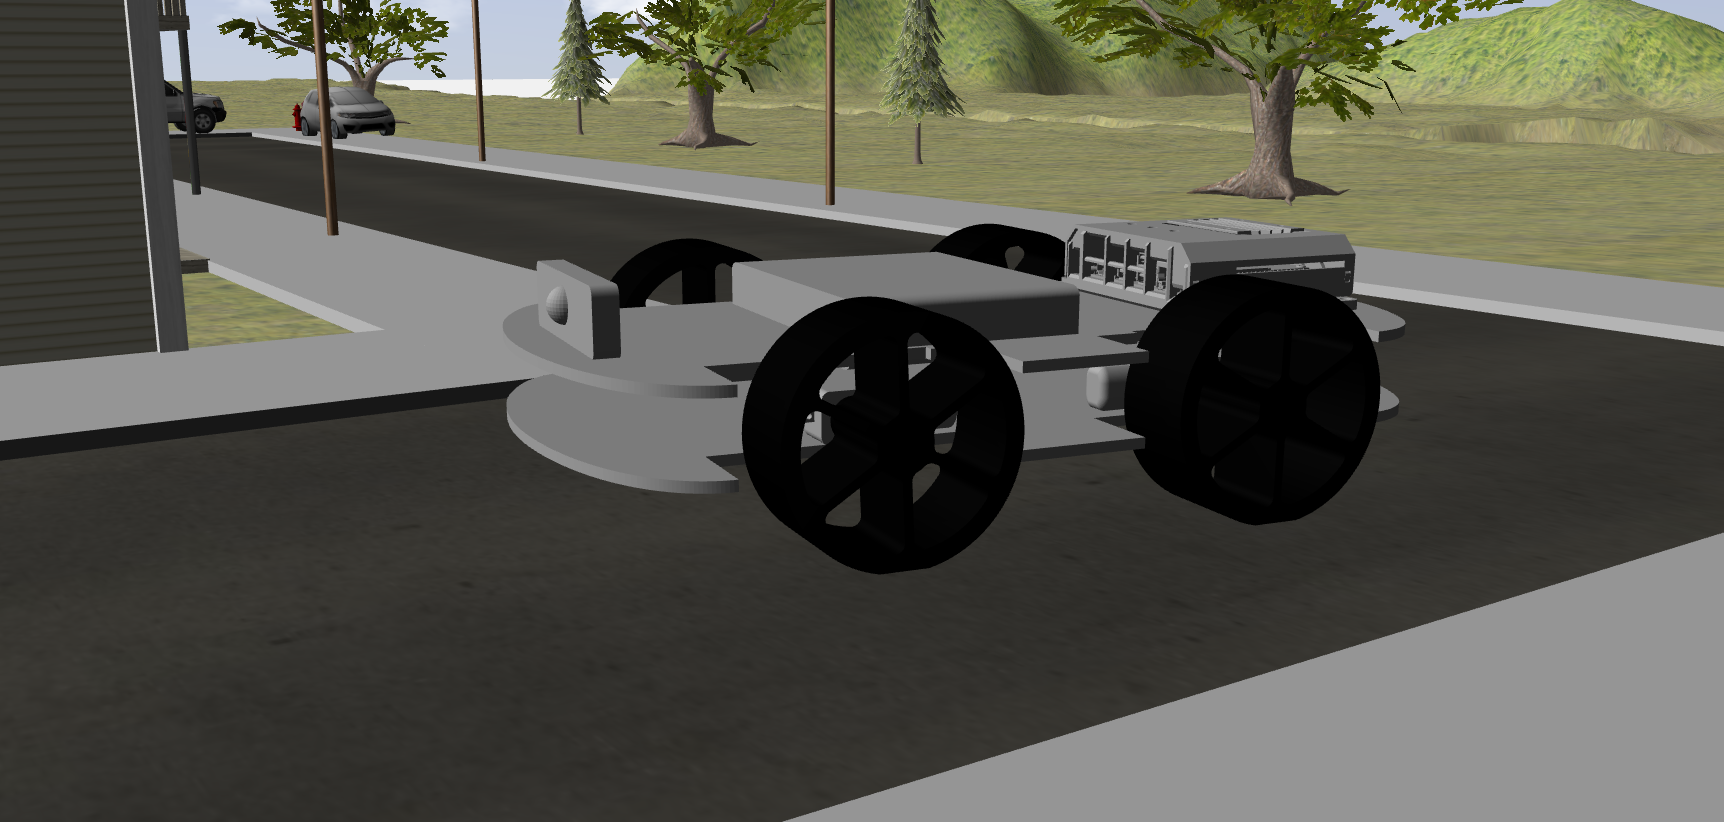
\includegraphics[width=12cm]{figs/modelGazebo}
	\end{center}
	\caption{Modelo dinámico del robot en \textit{Gazebo}.}
	\label{fig:modelGazebo}
\end{figure}\

\subsection{Seguimiento de carril}
\label{subsection:lanefollower}
\footnote{\url{https://github.com/jmvega/tfg-amariscal/src/......... interactive_regression_ros}}
Como se explicó en el Capítulo 2, la biblioteca elegida para realizar el seguimiento de carril, es \textit{JetRacer} tal y como se expuso en la Sección \ref{subsection:jetracer}. Dicha biblioteca se basa en la utilización de una red \textit{ResNet-18} preentrenada, consistente en una red neuronal convolucional de 18 capas, sobre la que a su vez, se entrena con un \textit{dataset} de un escaso mínimo número de imágenes. Proporciona diversos \textit{notebooks} de \textit{Jupyter} que hacen más la sencilla la obtención del \textit{dataset}, el entrenamiento y el ajuste del controlador.\\

El primer paso es la obtención del \textit{dataset} para posteriormente entrenar la red. Para ello, es necesario asociar cada imagen con el centro del carril, definido a partir de una coordenada en x y otra en y. La librería utiliza un \textit{widget} para \textit{Jupyter} llamado \textit{Jupyter Clickable Image Widget\footnote{\url{https://github.com/jaybdub/jupyter_clickable_image_widget}}} lo que permite que al hacer click sobre la imagen recibida a partir de un flujo de vídeo, esta se guarde con un nombre atendiendo al siguiente formato: \textit{x\_y\_identificador\_unico.jpg}. Es importante entrenar también con imágenes donde el ángulo del giro del robot sea elevado, tal y como muestra la Figura \ref{fig:traineddifficult} ya que de esa forma el robot sabrá reaccionar ante situaciones difíciles.\\

\begin{figure} [h!]
	\begin{center}
		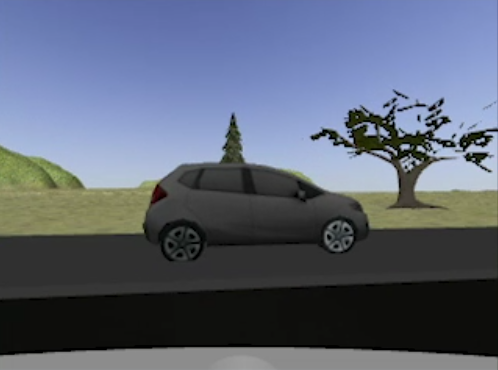
\includegraphics[width=6cm]{figs/trainedDifficult}
	\end{center}
	\caption{Imagen del \textit{dataset} donde el ángulo de giro necesario es elevado.}
	\label{fig:traineddifficult}
\end{figure}\

Para mover el robot dentro del simulador es necesario utilizar los controladores de los motores anteriormente desarrollados y para mayor comodidad, se realizó un control manual a través de una interfaz con \textit{PyQT} que se detallará en la Sección \ref{subsection:interface}.\\

Una vez obtenido el \textit{dataset}, se descarga el modelo preentrenado \textit{ResNet-18} utilizando la librería \textit{Torchvision} y se realiza una conversión para aprovechar los núcleos de la tarjeta gráfica mediante la plataforma \textit{CUDA} a través de la función \verb|to(device)| donde \verb|device| es \verb|torch.device('cuda')|.\\

El siguiente paso es el entrenamiento de la red. Para ello, en cada \textit{epoch} se calcula el error cuadrático medio, \textit{mean squared error (MSE loss)} entre una de las imágenes del \textit{dataset} y la salida actual de la red. Una vez calculado este error se realiza la propagación hacia detrás, \textit{backpropagation}, consistente en la propagación de los errores desde la capa de salida hasta la primera capa. Además se realiza una optimización de los pesos a través del algoritmo \textit{Adam} \cite{adam}, el cual es un método de optimización estocástica basado en el cálculo de las tasas individuales adaptables de entrenamiento, \textit{individual adaptive learning rates} a partir de estimaciones del primer y segundo momento del gradiente.\\

Para realizar el entrenamiento hay que fijar un número de \textit{epochs} que será el momento en el que el entrenamiento finalizará. En cada \textit{epoch} el error va bajando hasta llegar a un valor cercano a 0, dependiendo del número de imágenes del \textit{dataset} el tiempo invertido en realizar una \textit{epoch} será mayor o menor. En el caso del entrenamiento realizado, en 10 \textit{epochs} el error alcanzó el valor de 0.0117 tal y como representa la Figura \ref{fig:epochsimulator}.\\

\begin{figure} [h!]
	\begin{center}
		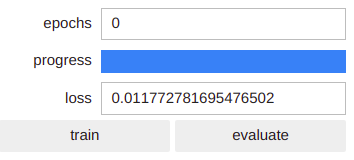
\includegraphics[width=8cm]{figs/epochSimulator}
	\end{center}
	\caption{Valor del error al finalizar el entrenamiento en el entorno simulado.}
	\label{fig:epochsimulator}
\end{figure}\

Tanto el entrenamiento como la ejecución de la red neuronal recibe imágenes de una baja resolución, 240 píxeles, ya que está diseñada para funcionar en placas de bajas prestaciones. Tras realizar el entrenamiento se genera un modelo \textit{.pth}. Para poder obtener la salida de la red es necesario pasar como argumento al modelo, el resultado de la función \verb|preprocess(image)|, que devuelve un tensor a partir de una imagen en formato \verb|numpy.ndarray|, tal y como se observa en el Código \ref{cod:lane}. Tras obtener la salida es posible representar el centro del carril con el resultado de la Figura \ref{fig:outputnnsim}.\\

\begin{code}[h]
	\begin{lstlisting}[language=Python]
			image = camera.read()
    		preprocessed = preprocess(image)
    		output = model(preprocessed).detach().cpu().numpy().flatten()
	\end{lstlisting}
	\caption[Obtención de la salida de la red neuronal \textit{ResNet-18}.]{Obtención de la salida de la red neuronal \textit{ResNet-18}.}
	\label{cod:lane}
\end{code}

\begin{figure} [h!]
	\begin{center}
		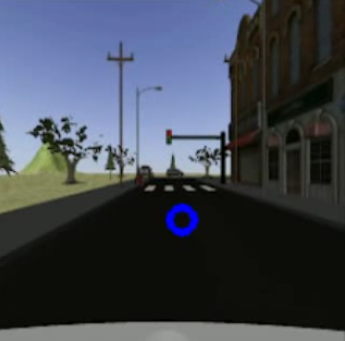
\includegraphics[width=6cm, height=5cm]{figs/outputNNsim}
	\end{center}
	\caption{Salida de la red neuronal \textit{ResNet-18} en el simulador \textit{Gazebo}.}
	\label{fig:outputnnsim}
\end{figure}\

En el caso del simulador y al ser una plataforma de pruebas, el objetivo principal es entrenar la red y probar su efectividad en un entorno simulado, y no desarrollar un controlador a partir de la salida de la red. Por lo que el seguimiento del carril se realizará mediante un autómata que recorrerá la ciudad de forma que se pueda observar el comportamiento de la red neuronal.\\

\subsection{Detección de objetos}
\label{subsection:objectdetector}
La detección de objetos se ha llevado a cabo mediante una red neuronal convolucional llamada \textit{YOLO V3 Tiny} debido a su gran rendimiento en placas de reducida potencia. La versión \textit{Tiny-YOLO} reduce el número de capas y precisión de detección pero aumenta la tasa de \textit{FPS} por lo que es muy conveniente su uso en dispositivos como \textit{NVIDIA Jetson Nano}. Existen distintas versiones de \textit{Tiny-YOLO}. La tercera versión cuenta con 15 capas convolucionales\footnote{\url{https://github.com/pjreddie/darknet/blob/master/cfg/yolov3-tiny.cfg}} a diferencia de la cuarta que cuenta con 29 capas\footnote{\url{https://github.com/AlexeyAB/darknet/blob/master/cfg/yolov4-tiny.cfg}}. En el Cuadro \ref{table:v3vsv4} se puede observar una comparación entre ambas versiones de la red con una resolución de 416 píxeles, extraída de la siguiente fuente\cite{versus}, que arroja como resultado un mejor rendimiento en la tercera versión, si bien es cierto que atendiendo al artículo de \textit{YOLO V4} \cite{yolov4} la precisión de la red ha sido incrementada en un 10\% en decremento de la tasa de \textit{FPS}.\\

\begin{table}[H]
	\begin{center}
		\begin{tabular}{|c|c|c|}
			\hline
			\textbf{Placa}     & \textbf{YOLO V3 Tiny} & \textbf{YOLO V4 Tiny}
			\\
			\hline
			NVIDIA Jetson Nano & 15                    & 7.8
			\\
			NVIDIA Jetson TX2  & 19                    & 11.5
			\\
			NVIDIA AGX Xavier  & 32                    & 22
			\\
			\hline
		\end{tabular}
		\caption{\textit{FPS} obtenidos en diferentes placas \textit{NVIDIA}}
		\label{table:v3vsv4}
	\end{center}
\end{table}

La ejecución de la simulación se ha realizado utilizando una tarjeta gráfica \textit{NVIDIA MX330}. Se trata de una tarjeta de gama baja y consumo reducido diseñada para portátiles. En cuanto a la decisión de la resolución de la imagen con la que trabaja la red neuronal se ha realizado una comparación disponible en el Cuadro \ref{table:versusnotebook}.\\

\begin{table}[H]
	\begin{center}
		\begin{tabular}{|c|c|}
			\hline
			\textbf{Resolución} & \textbf{FPS}
			\\
			\hline
			416 x 416           & 41.1
			\\
			608 x 608           & 21.6
			\\
			832 x 832           & 12.3
			\\
			\hline
		\end{tabular}
		\caption{FPS obtenidos en \textit{YOLO V3 Tiny} con la tarjeta gráfica \textit{NVIDIA MX330}}
		\label{table:versusnotebook}
	\end{center}
\end{table}

Se ha utilizado la red \textit{YOLO V3 Tiny} sobre \textit{Darknet ROS\footnote{\url{https://github.com/leggedrobotics/darknet_ros}}}. Se trata de un paquete que implementa \textit{Darknet} utilizando el \textit{framework ROS}. Su funcionamiento se basa en la recepción de la imagen a través de un \textit{topic} fijado en el fichero de configuración \textit{ros.yaml} y la publicación de objetos detectados mediante \textit{bounding boxes} en un \textit{topic} llamado \textit{/darknet\_ros/bounding\_boxes} en el que se publican mensajes con los datos del Código \ref{cod:boundingboxes}. De esa forma se puede extraer las coordenadas del \textit{bounding box}, el objeto detectado y su probabilidad. Existe un fichero \textit{YAML} en el que se especifican los objetos a detectar y en el que es necesario especificar límite o \textit{threshold} debajo del cual el objeto detectado será descartado. En el caso del entorno simulado los colores son fijos y los objetos son muy genéricos por lo que el \textit{threshold} se pudo subir hasta 0.8. De esta forma se evitan falsos positivos y se consigue una detección mucho más fiable.\\

\begin{code}[h]
	\begin{lstlisting}
		float64 probability
		int64 xmin
		int64 ymin
		int64 xmax
		int64 ymax
		int16 id
		string Class
	\end{lstlisting}
	\caption[Contenido del mensaje \textit{BoundingBox}.]{Contenido del mensaje \textit{BoundingBox}.}
	\label{cod:boundingboxes}
\end{code}

De esta forma se pueden detectar objetos como semáforos, personas o coches tal y como se puede observar en la Figura \ref{fig:darknetsimulator}.\\

\begin{figure} [h!]
	\begin{center}
		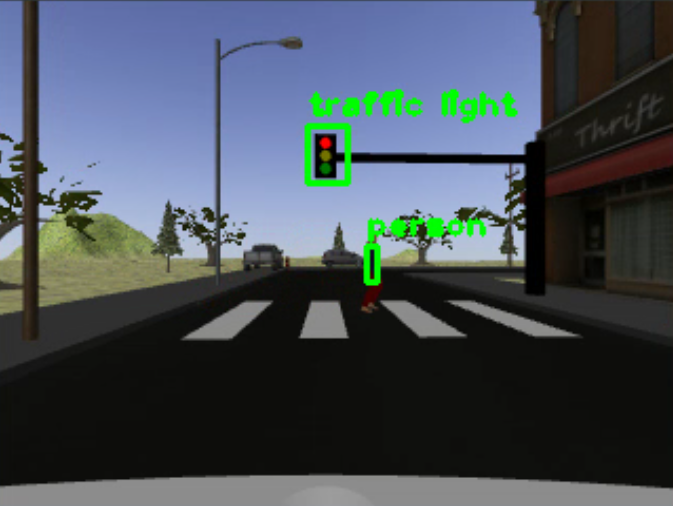
\includegraphics[width=6cm]{figs/darknetSimulator}
	\end{center}
	\caption{Salida de la red neuronal \textit{YOLO V3 Tiny} en el simulador \textit{Gazebo}.}
	\label{fig:darknetsimulator}
\end{figure}\

En el caso de la detección del semáforo es necesario tratar la imagen para detectar el color. Para ello, se extrae la imagen del \textit{bounding box} mediante sus coordenadas, contenidas en el mensaje tal y como consta en el Código \ref{cod:boundingboxes}, se transforma al espectro \textit{HSV} con el objetivo de posteriormente realizar un filtro de color. Al aplicar la máscara sobre una imagen en \textit{HSV} y no en \textit{RGB} obtenemos una detección de mayor fiabilidad, tal y como se puede observar en la Figura
\ref{fig:detector}.\\

\begin{figure} [h!]
	\begin{center}
		
\includegraphics[width=2cm, height=4cm]{figs/cropped}\hspace{2cm}
\includegraphics[width=2cm, height=4cm]{figs/hsv}\hspace{2cm}
\includegraphics[width=2cm,
			height=4cm]{figs/mask}
	\end{center}
	\caption{Detección del semáforo mediante transformación a \textit{HSV} y filtro de color.}
	\label{fig:detector}
\end{figure}\

El robot se detiene al detectar el semáforo en rojo y en el momento que cambie a verde reanuda la marcha. En el caso de detectar una señal de stop se parará durante 5 segundos.
Todo ello se puede observar en capturas de la ejecución representadas en la Figura \ref{fig:simexecution}.\\

\begin{figure} [h!]
	\begin{center}
		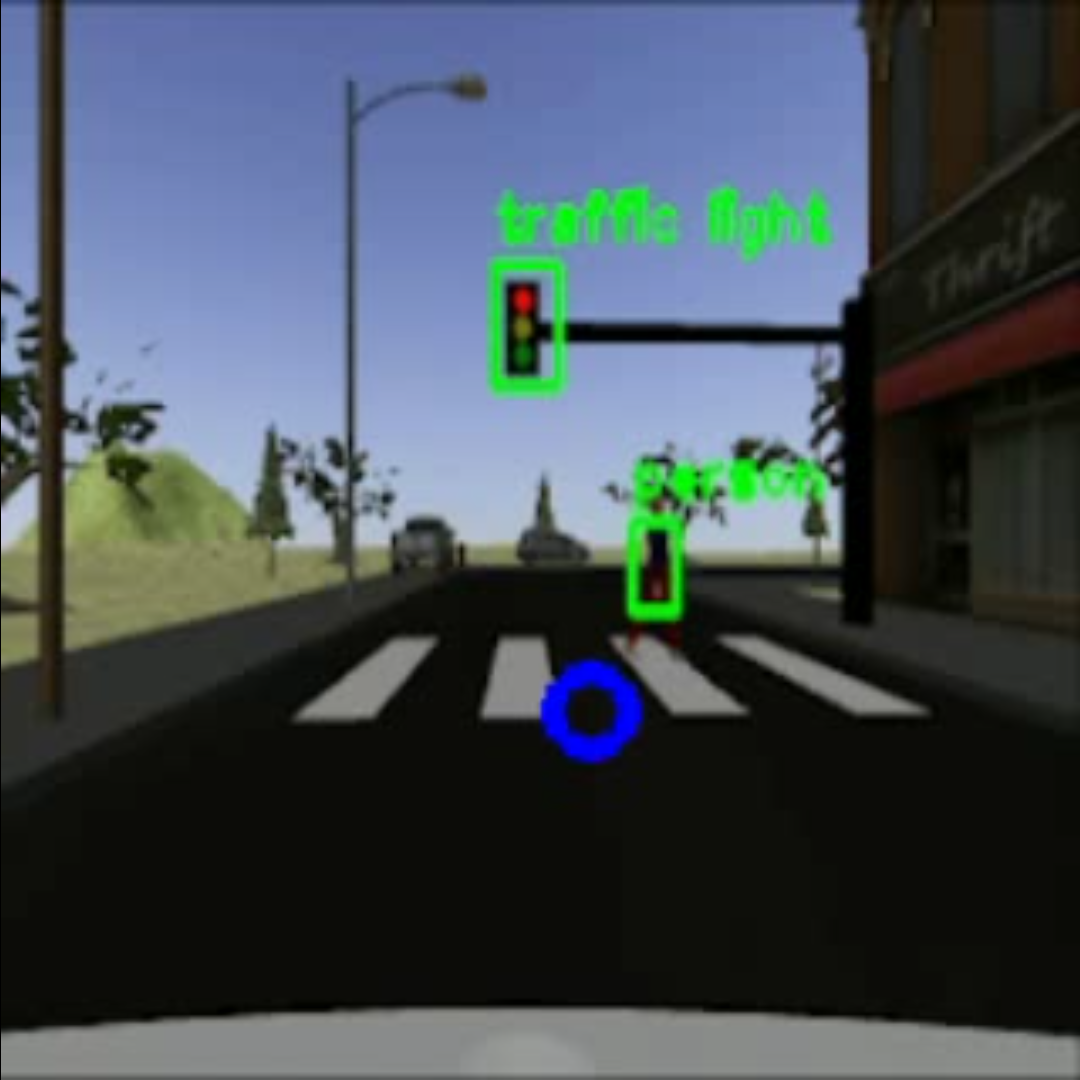
\includegraphics[width=5cm]{figs/simRed}\hspace{0.1cm}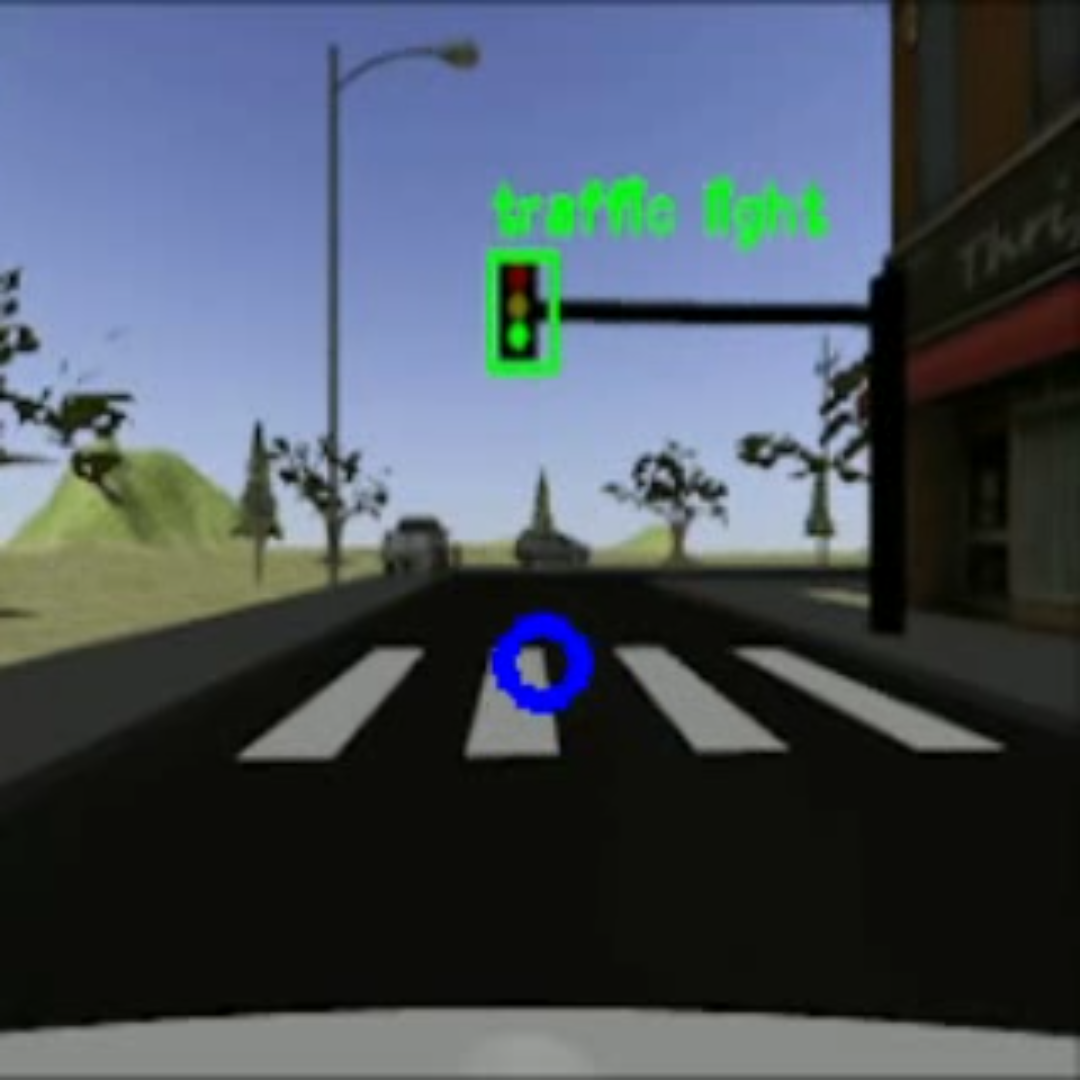
\includegraphics[width=5cm]{figs/simGreen}\hspace{0.1cm}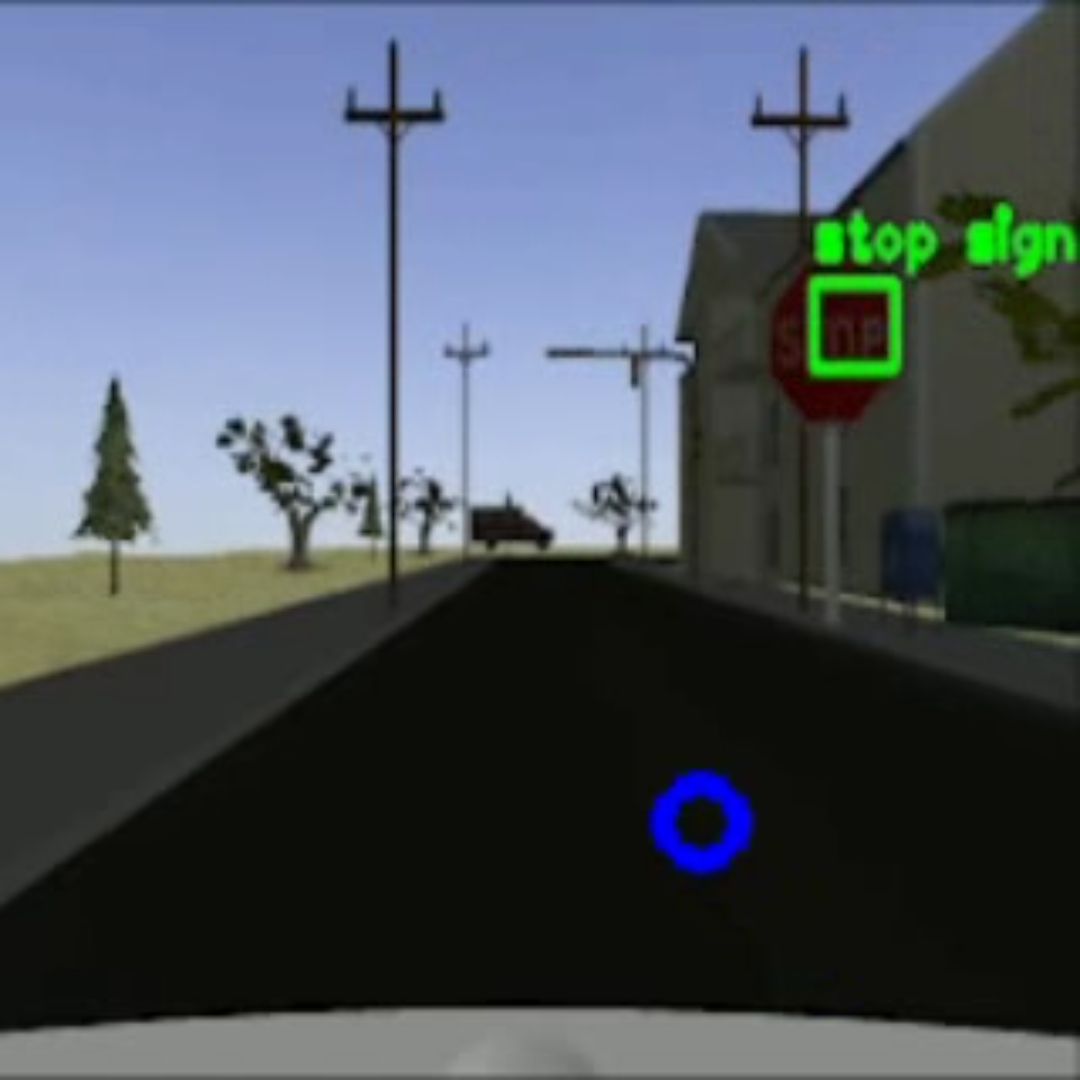
\includegraphics[width=5cm]{figs/simStop}
	\end{center}
	\caption{Capturas de la ejecución con dos redes neuronales.}
	\label{fig:simexecution}
\end{figure}\

\subsection{Interfaz de usuario}
\label{subsection:interface}
Con el objetivo de realizar un control sencillo de la simulación se ha realizado una interfaz gráfica desarrollada con la biblioteca \textit{PyQT}. Dicha interfaz dispone de una cruceta para realizar un control manual del robot. Incluye también un botón para iniciar la simulación y otro para reiniciarla, de modo que, el robot vuelve al punto inicial. Así como un botón para activar las dos cámaras. Dispone de una cámara alojada en el propio robot llamada \textit{onboard} y otra que se desplaza cuando el robot avanza de modo que aporta una visión del recorrido que realiza el robot. La interfaz descrita se puede observar en la Figura \ref{fig:gui}.\\

\begin{figure} [h!]
	\begin{center}
		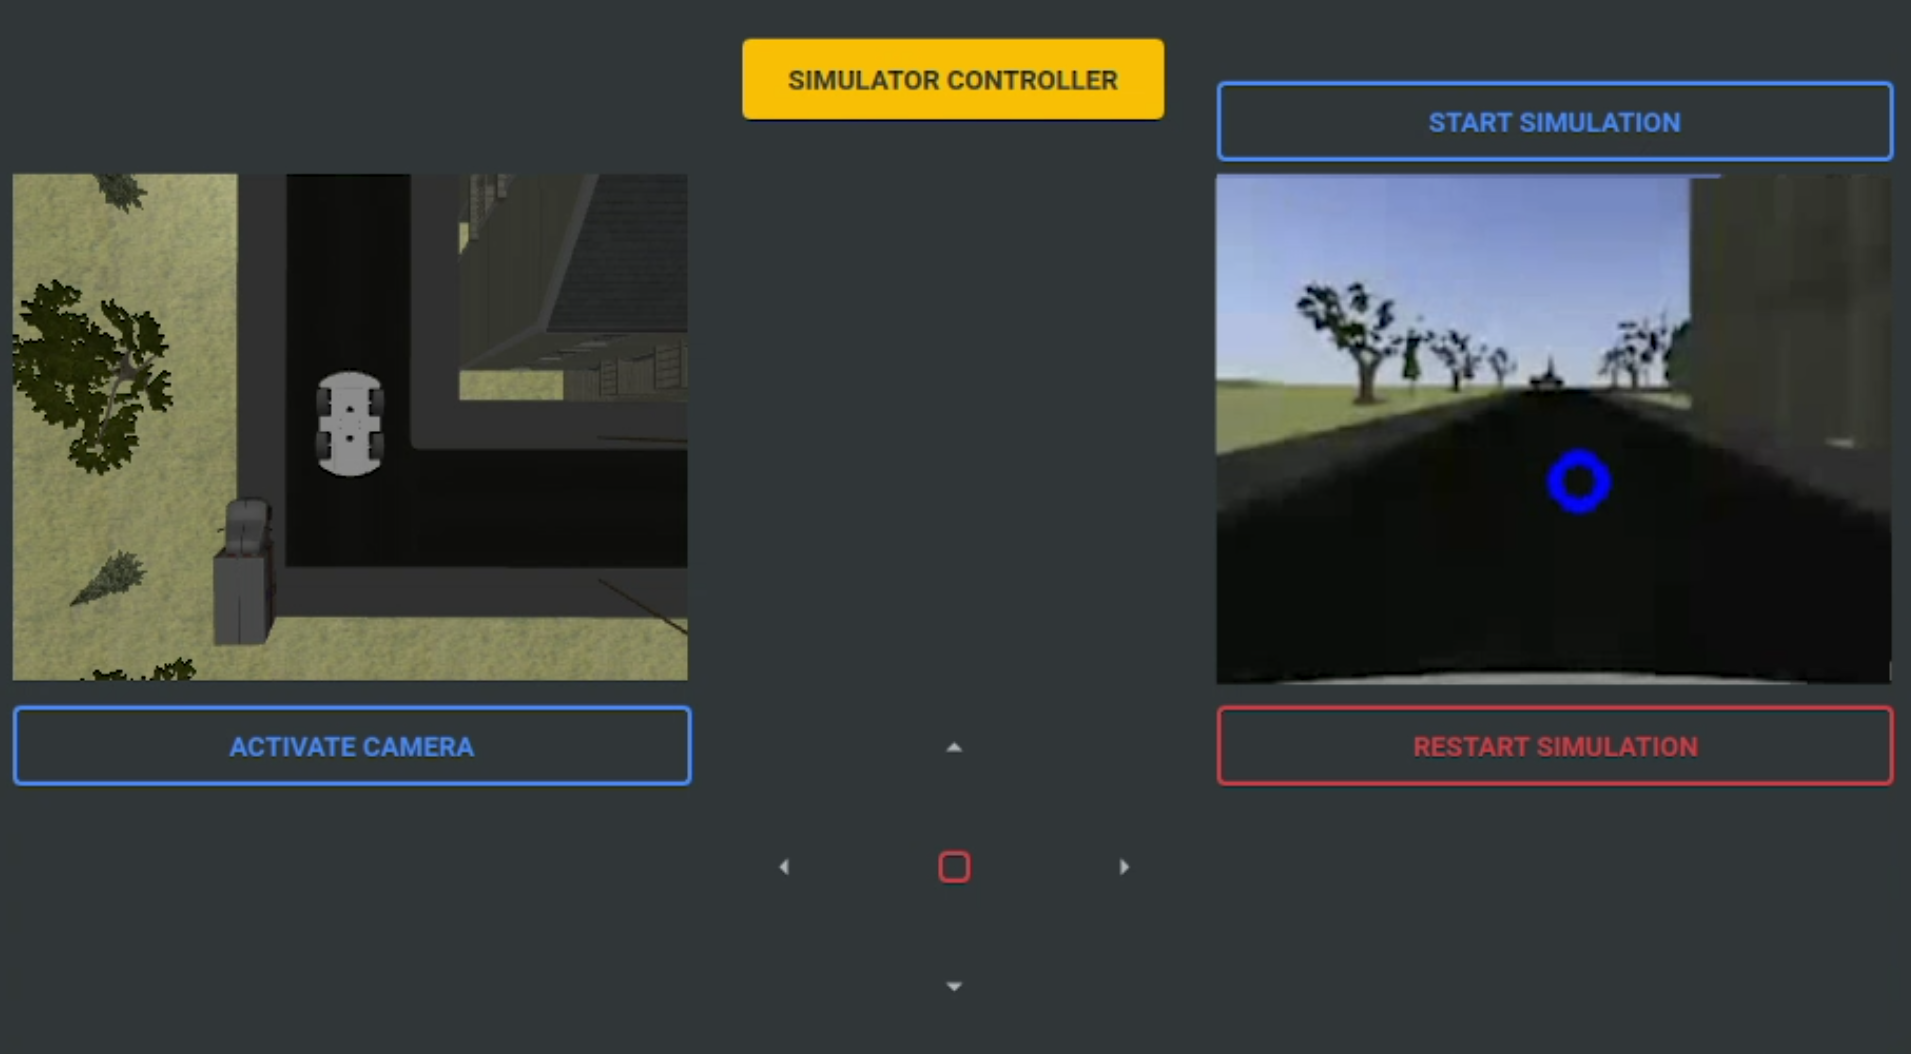
\includegraphics[width=10cm]{figs/GUI}
	\end{center}
	\caption{Interfaz de usuario desarrollada para controlar la simulación.}
	\label{fig:gui}
\end{figure}\

\section{Entorno real}
\label{section:real}
En esta sección se exponen los elementos utilizados para componer un entorno real en el que un robot, representado en la Figura \ref{fig:realrobot}, equipado con una cámara como sensor principal circula reaccionando ante objetos estáticos y dinámicos. Así como las particularidades del sistema a la hora de realizar la transición desde el entorno simulado al real.\\

\begin{figure} [h!]
	\begin{center}
		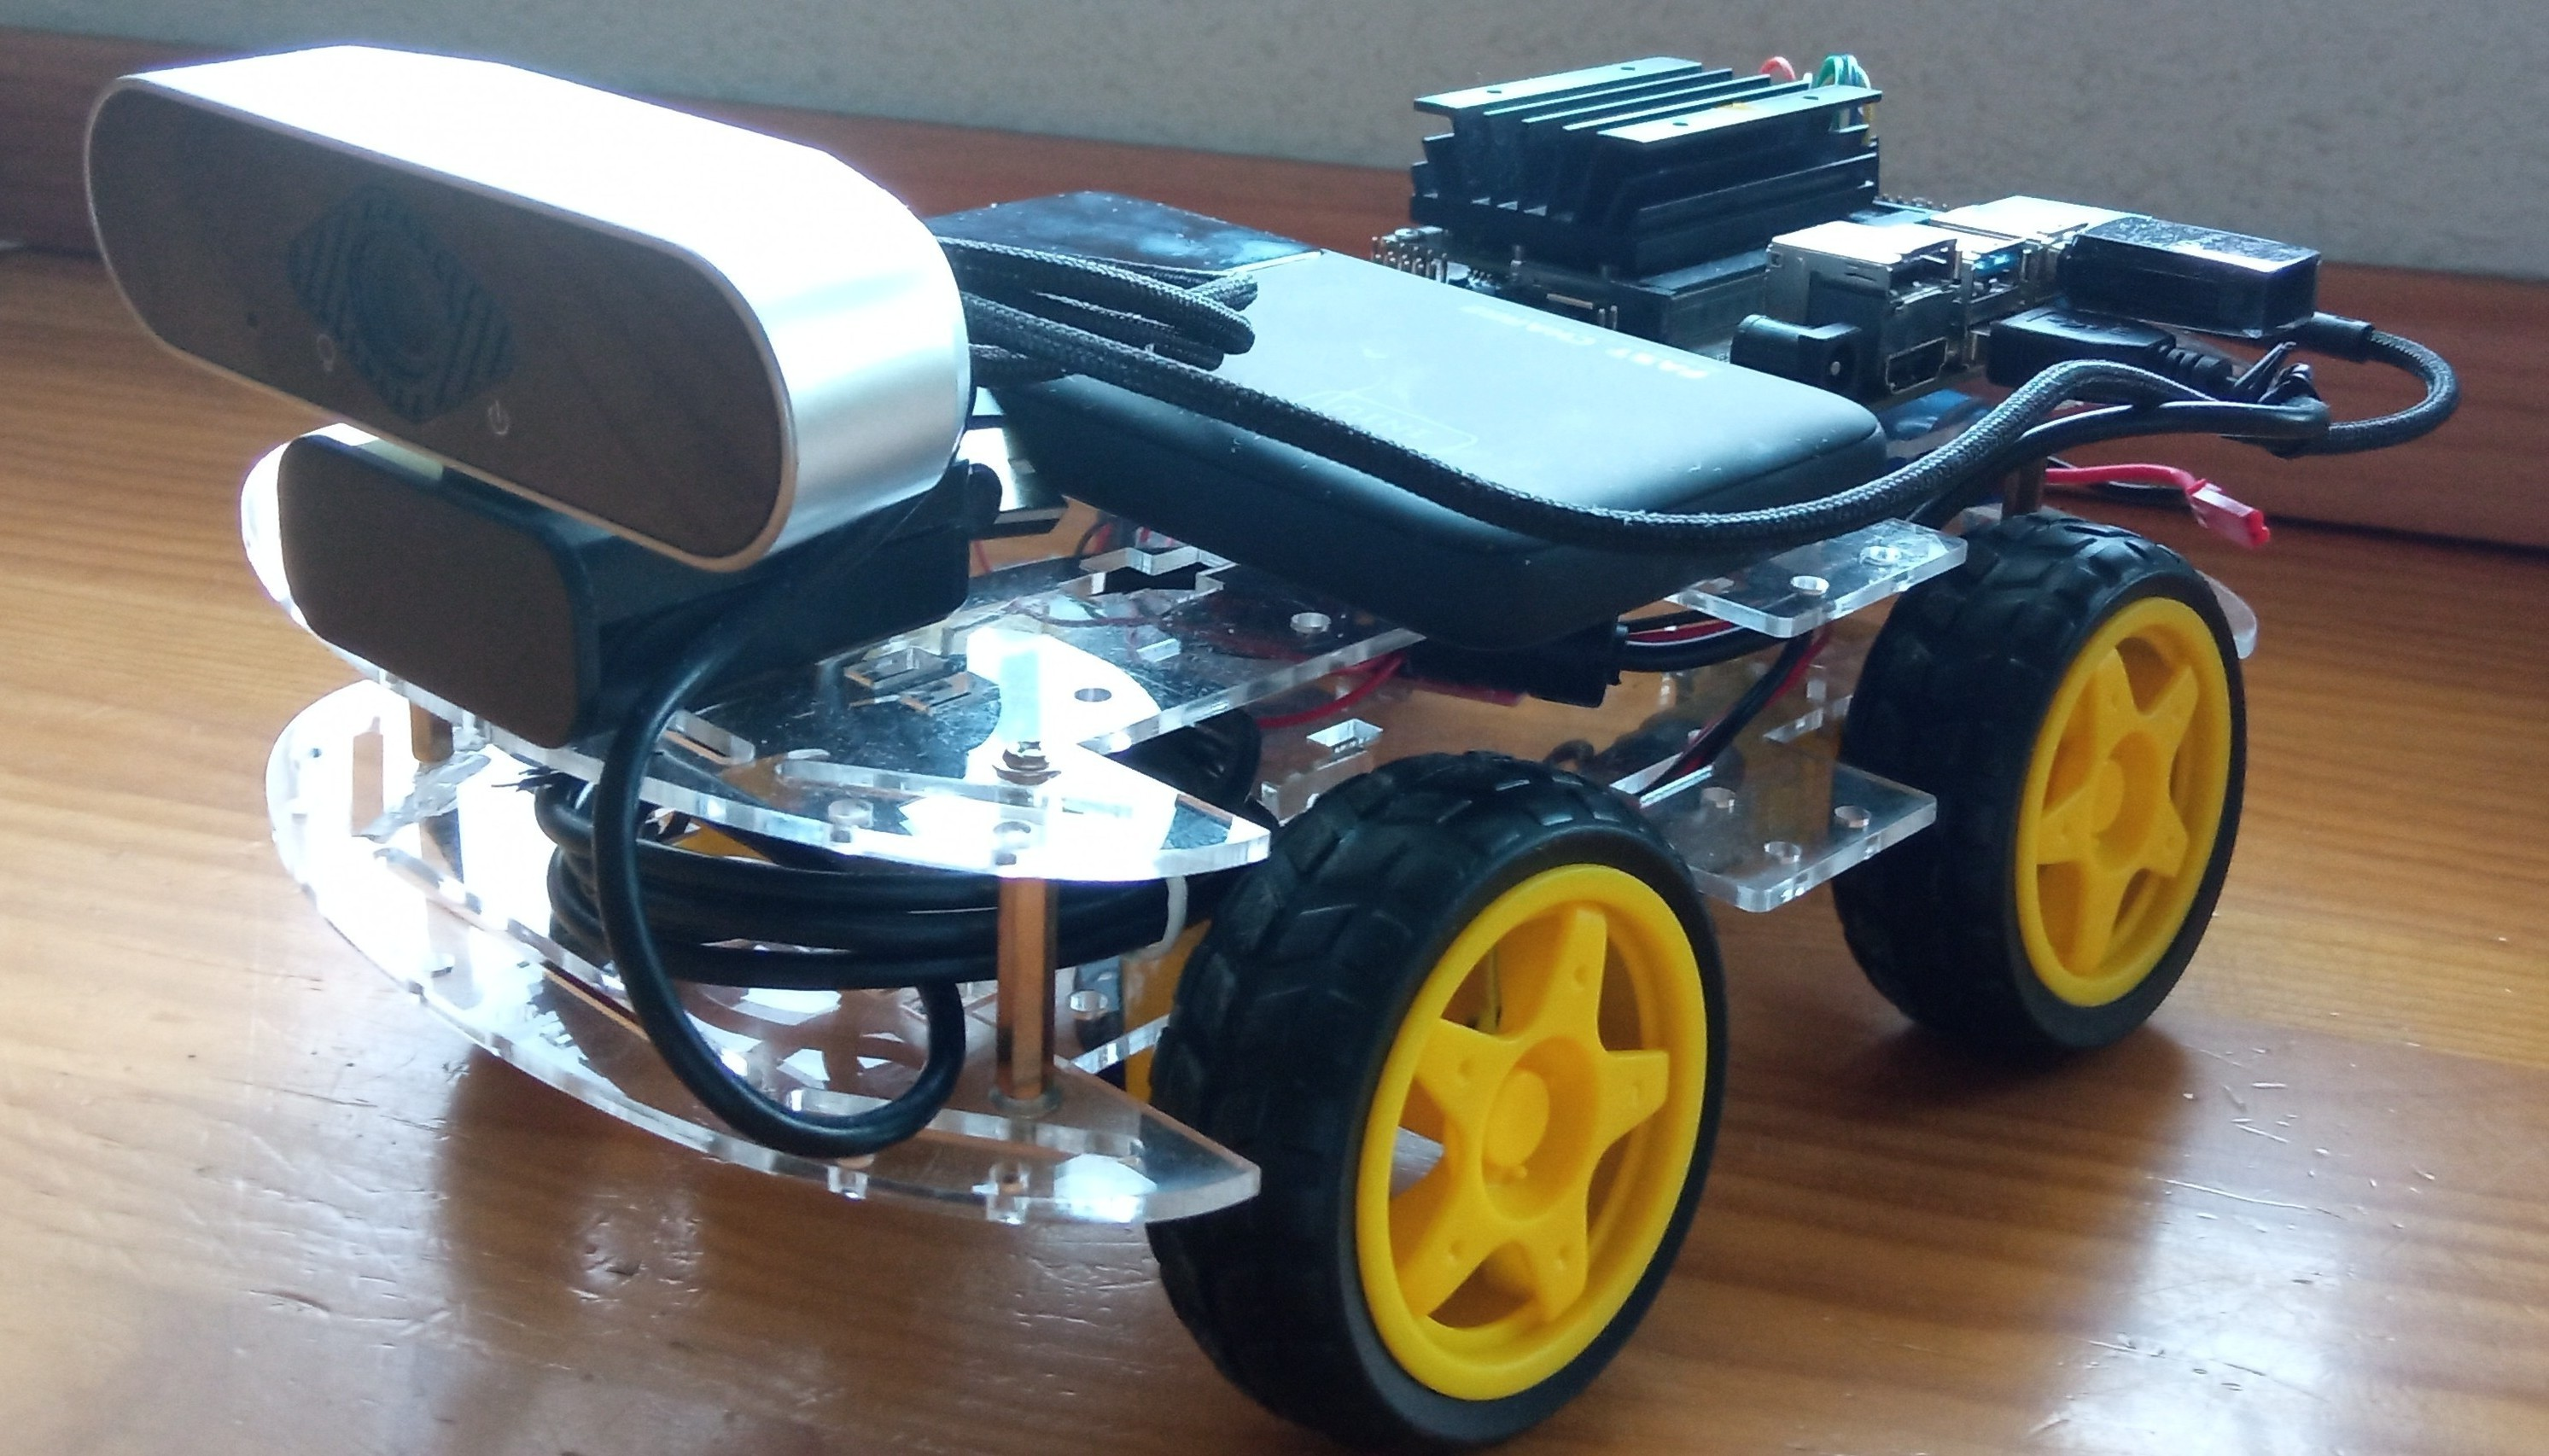
\includegraphics[width=10cm]{figs/robot}
	\end{center}
	\caption{Robot con \textit{NVIDIA Jetson Nano}.}
	\label{fig:realrobot}
\end{figure}\

\subsection{Objetos}
El entorno real se compone de diversos objetos; un circuito elaborado con pistas Scalextric sobre el que se sitúan objetos como un semáforo dinámico que cambia de color en un modo automático cada cierto tiempo, una señal de stop y un peatón. Dichos objetos se pueden observar en la Figura \ref{fig:objects}.\\

\begin{figure} [h!]
	\begin{center}
		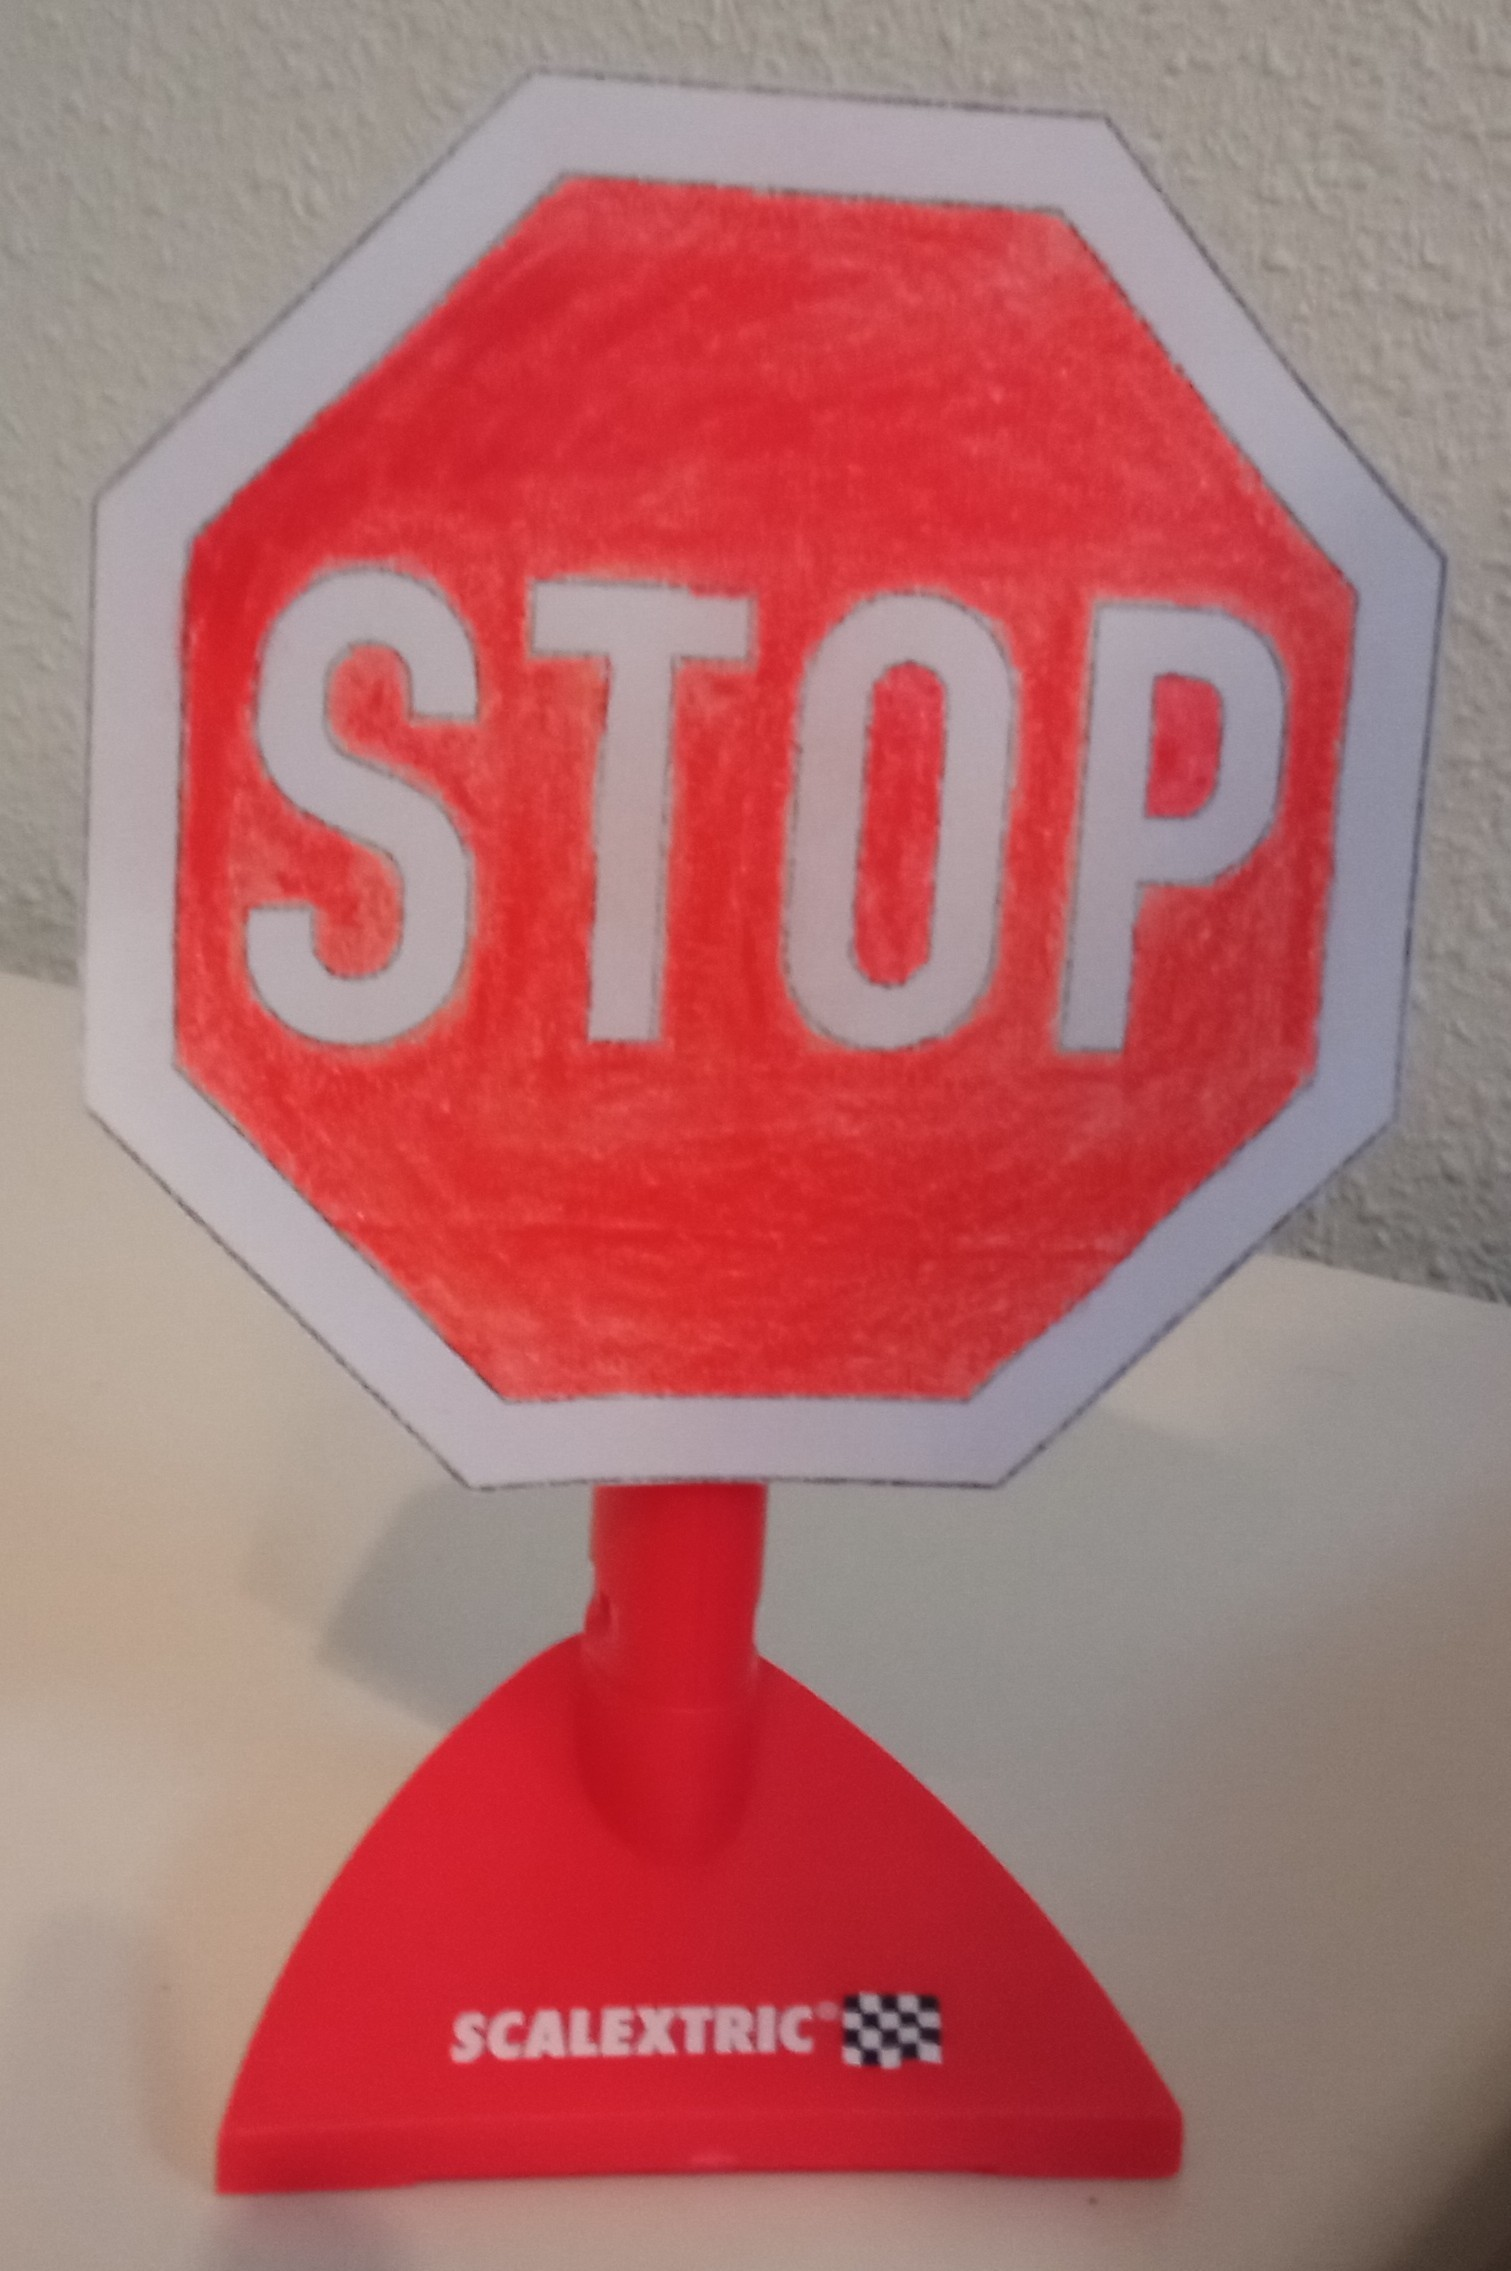
\includegraphics[width=4cm, height=5cm]{figs/realstopsign}\hspace{0.5cm}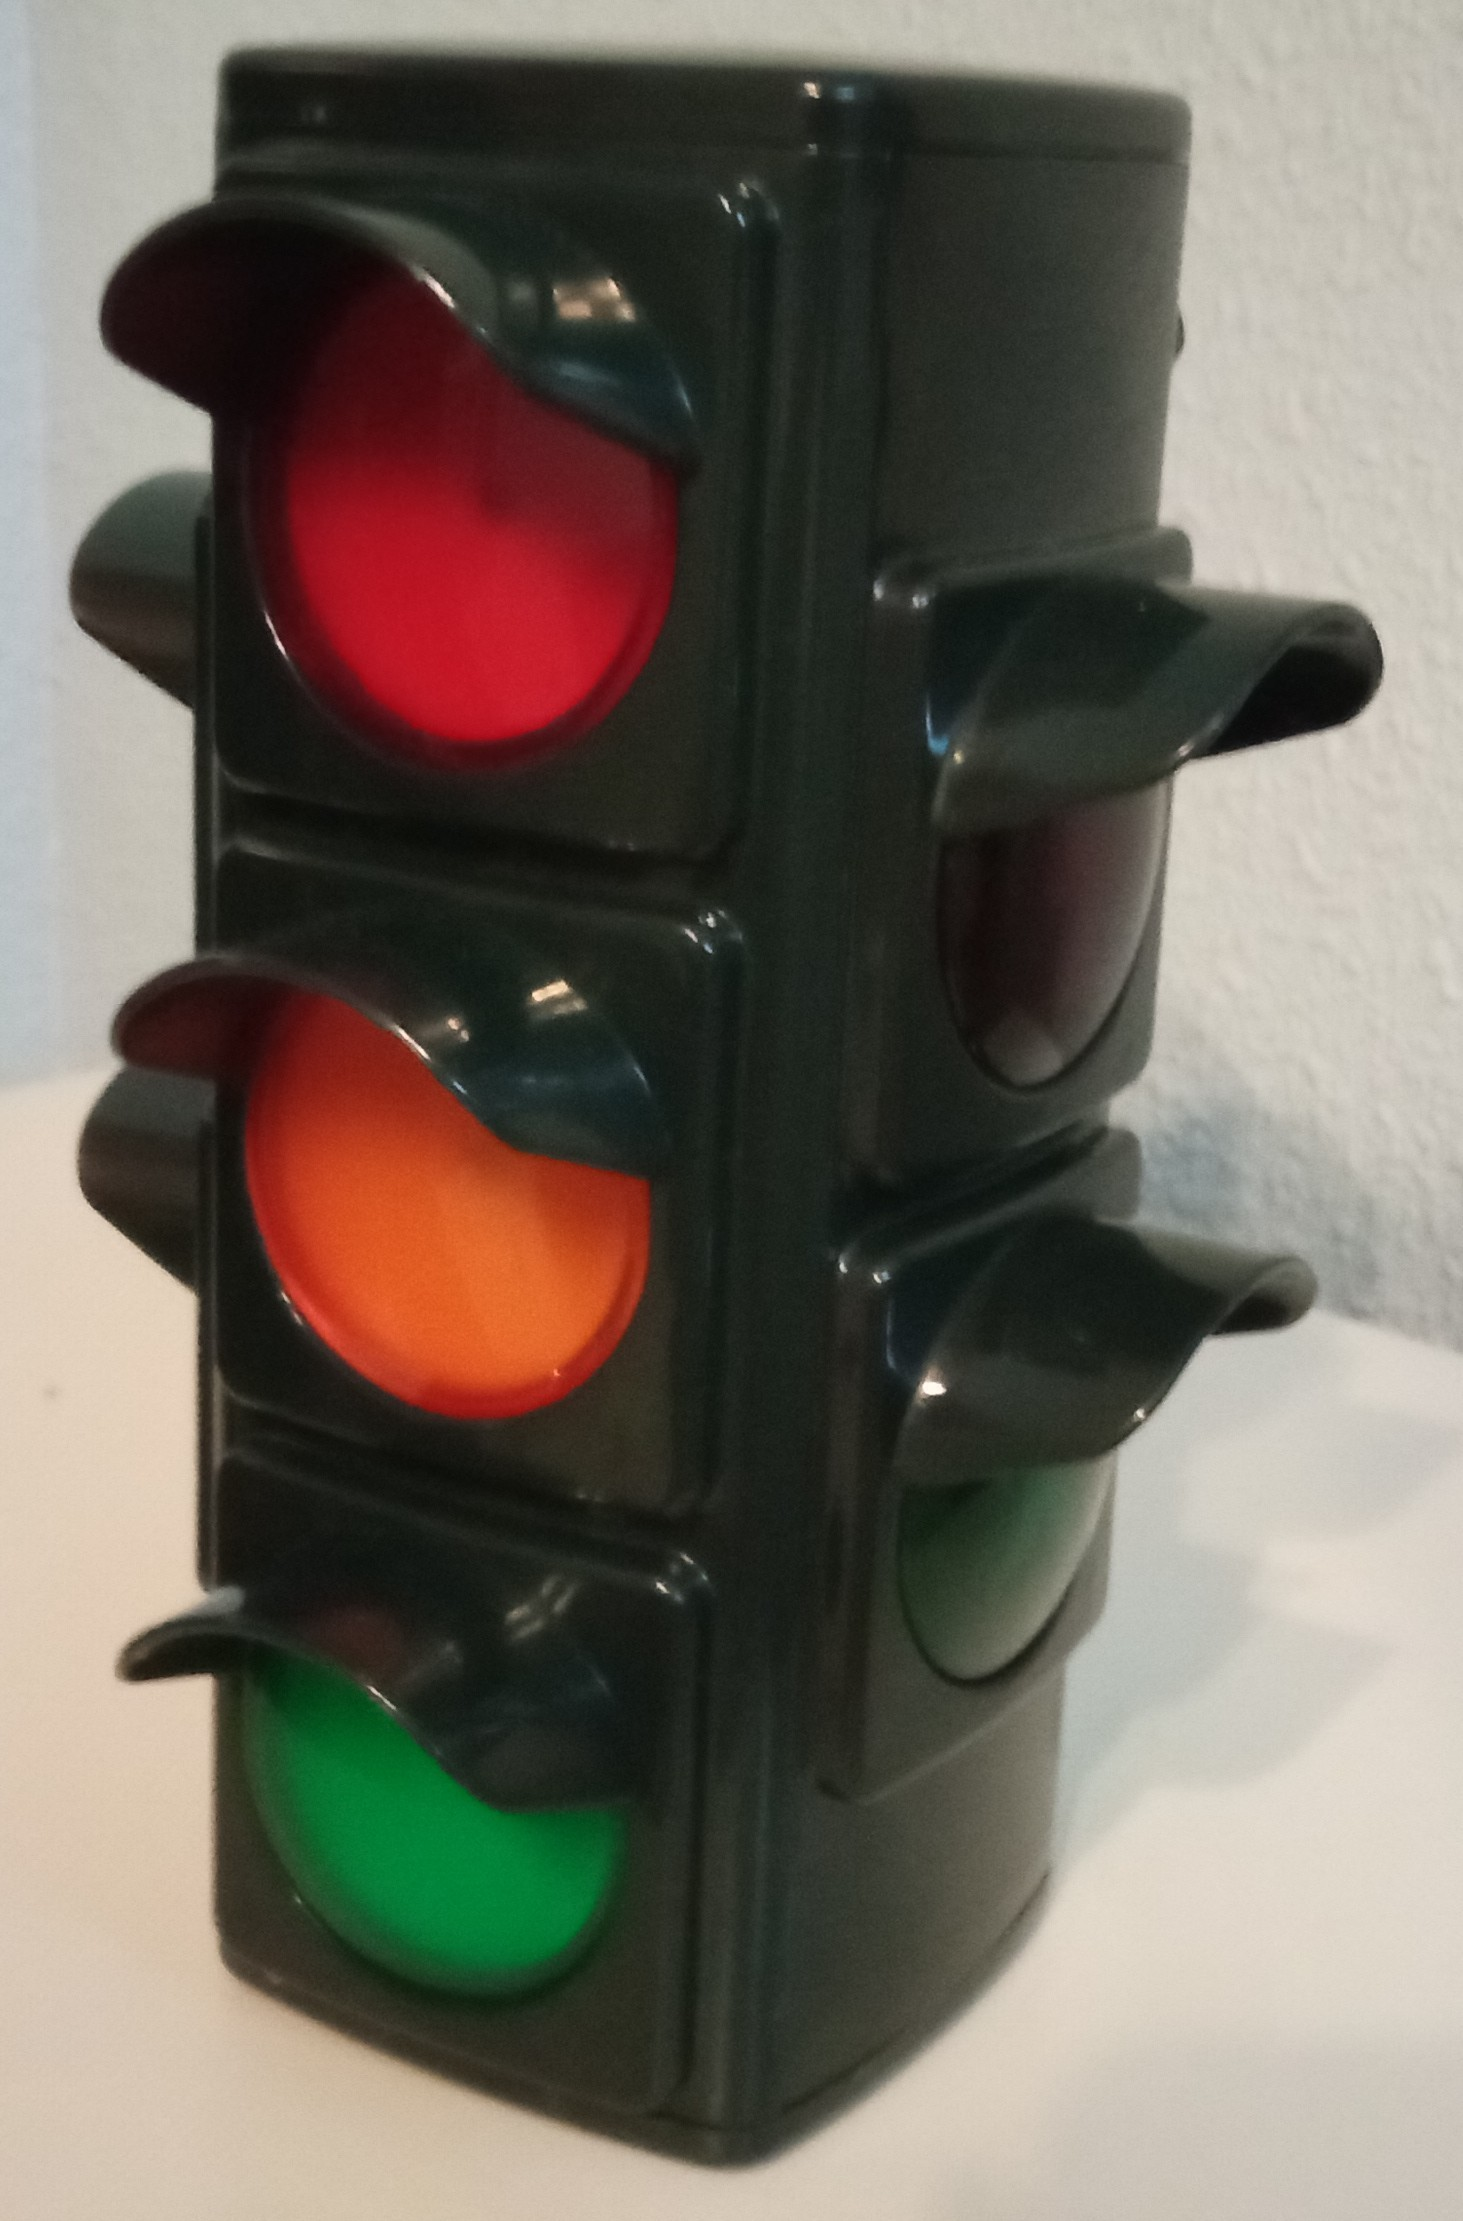
\includegraphics[width=4cm]{figs/realtrafficlight}\hspace{0.5cm}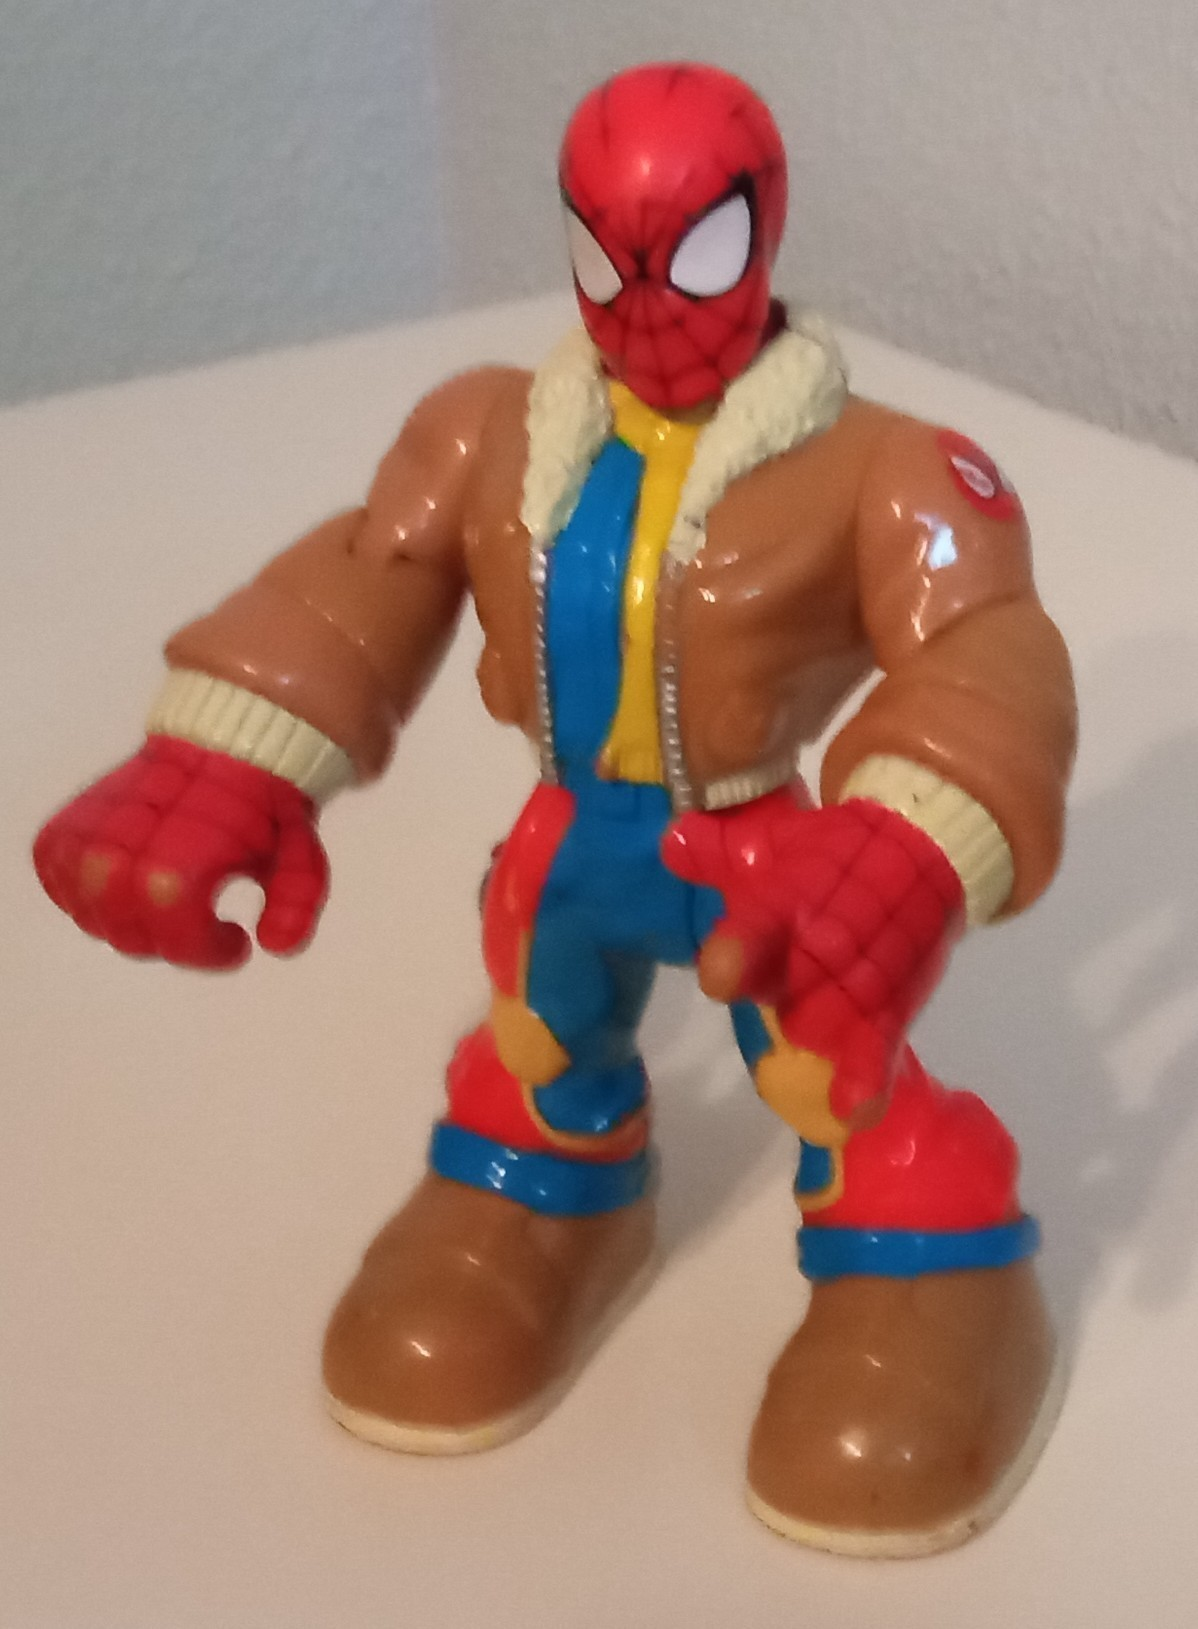
\includegraphics[width=4cm, height=5cm]{figs/realpedestrian}
	\end{center}
	\caption{Objetos reales dinámicos y estáticos.}
	\label{fig:objects}
\end{figure}\

\subsection{Circuito}
En principio se construyó un circuito inicial, representado en la Figura \ref{fig:circuit}, en el que se entrenó la red neuronal de seguimiento de carril. Posteriormente se fue agrandando en el espacio introduciendo rectas más largas para poder interactuar mejor con objetos.\\

\begin{figure} [h!]
	\begin{center}
		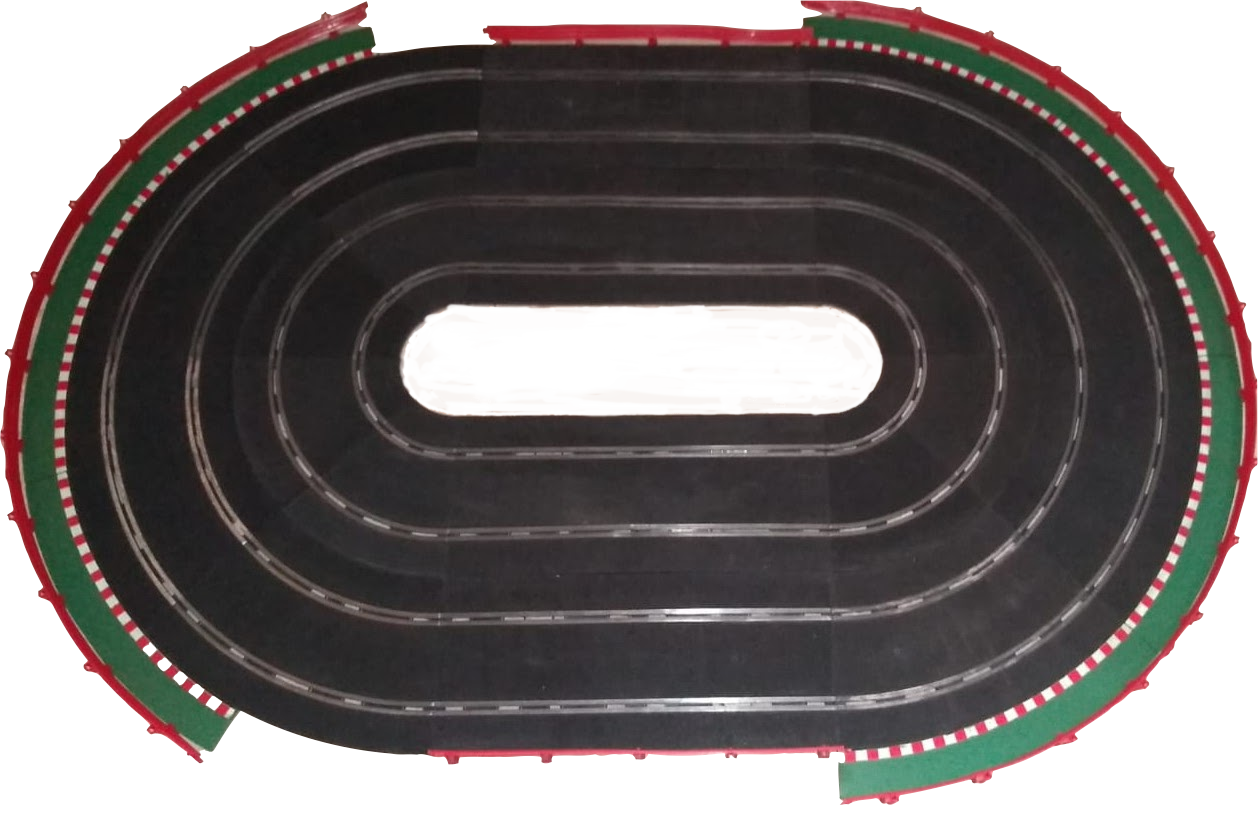
\includegraphics[width=8cm]{figs/circuit}
	\end{center}
	\caption{Circuito inicial construido a partir de pistas Scalextric.}
	\label{fig:circuit}
\end{figure}\

Tras ubicar todos los objetos alrededor del circuito, da como resultado la imagen representada en la Figura \ref{fig:circuitwithobjects}.\\

\begin{figure} [h!]
	\begin{center}
		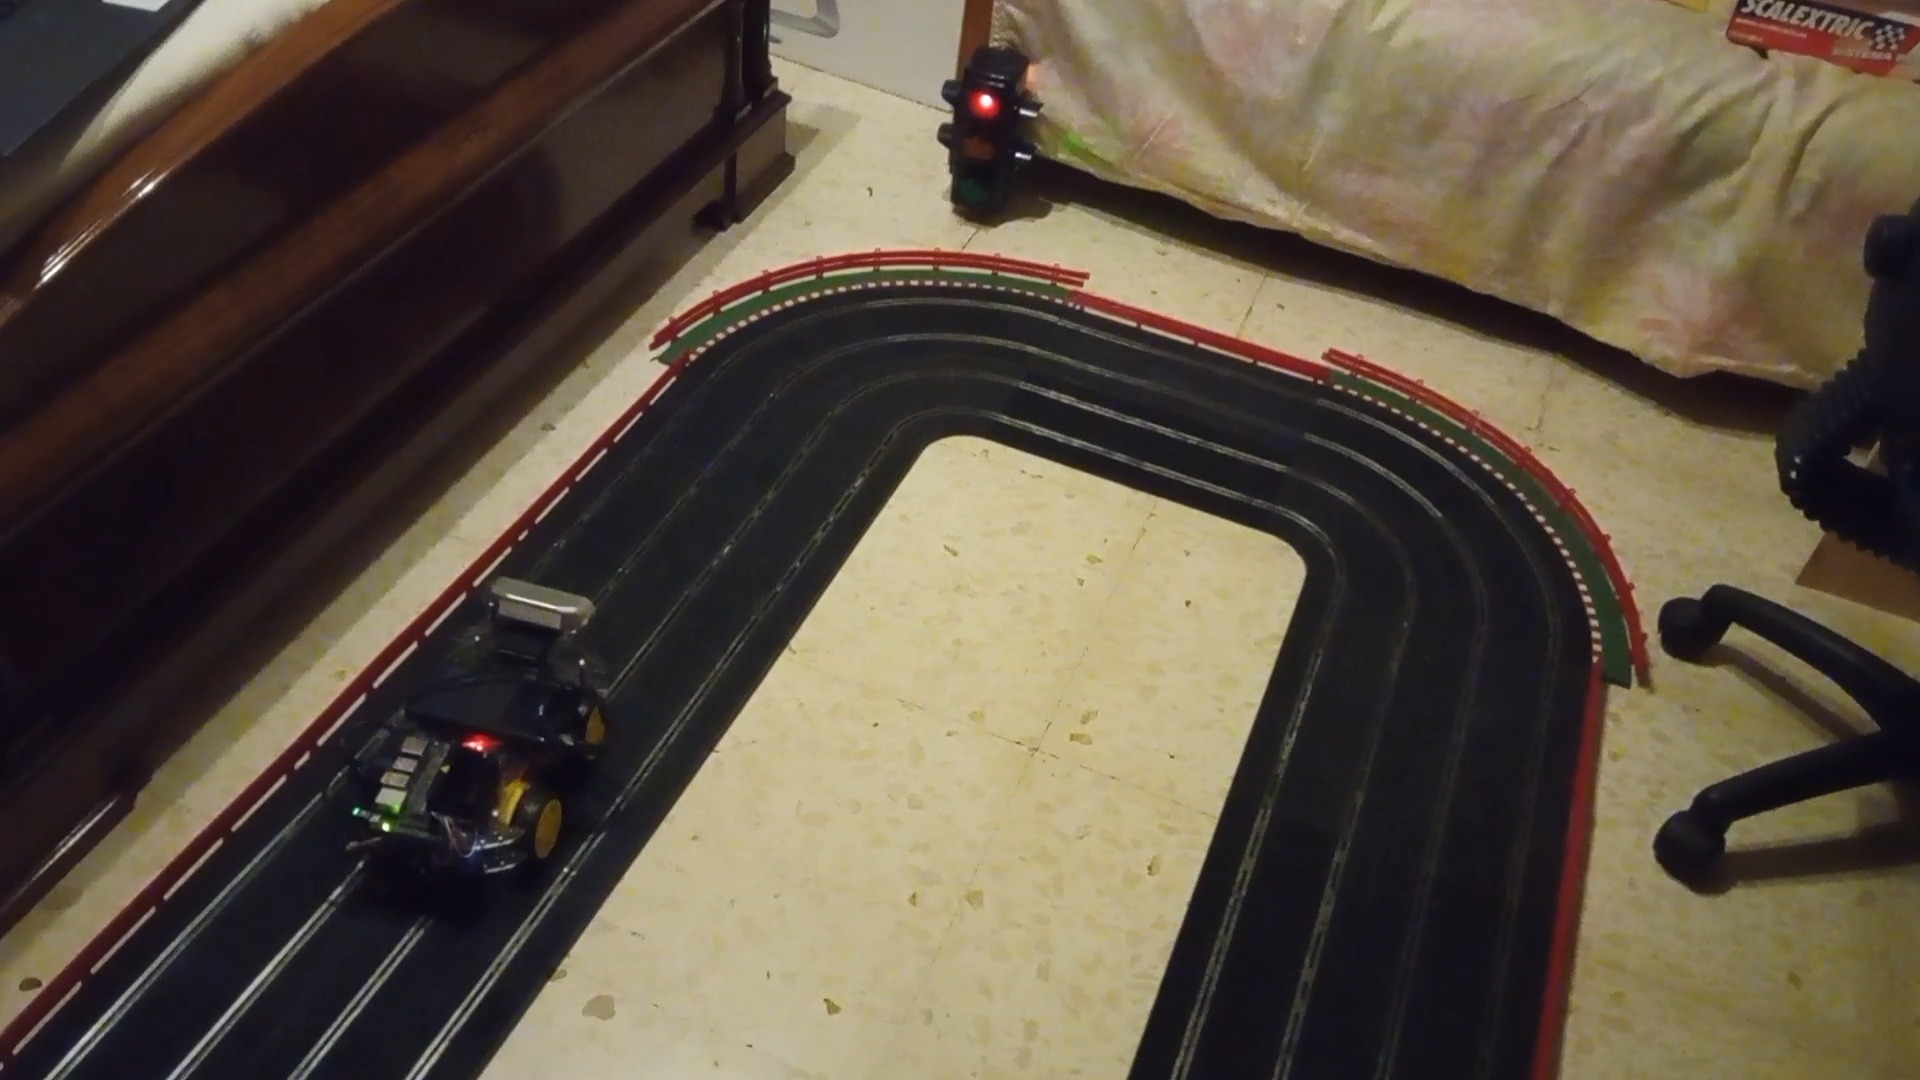
\includegraphics[width=12cm]{figs/circuitwithobjects}
	\end{center}
	\caption{Circuito con objetos.}
	\label{fig:circuitwithobjects}
\end{figure}\

\section{Redes neuronales en el entorno real}
El entrenamiento de la red neuronal \textit{ResNet-18} se realiza de igual forma que en el entorno simulado, la principal diferencia a tener en cuenta es la luz ambiente y los colores, que a diferencia del simulador, cambian dependiendo de como incida la luz. Por ello, es interesante comprobar el comportamiento de la red neuronal cuando hay cambios de luz. Además, existen multitud de diferencias entre una luz artificial y la luz natural, cuando se trabaja con luz natural es necesario tener en cuenta la incidencia que los rayos del sol pueden hacer sobre la lente de la cámara. Por ello se decidió entrenar la red con luz artificial, con imágenes como la que representa la Figura \ref{fig:imagedataset}, obteniendo el valor de 0.0034 como error. La librería \textit{JetRacer} recomienda entrenar la red con un mínimo de 50 imágenes\footnote{\url{https://github.com/NVIDIA-AI-IOT/jetracer/blob/master/docs/examples.md}}, por lo que se decidió entrenar con 100 imágenes para que el tiempo de entrenamiento no fuese demasiado elevado y no provocara un aumento muy grande de temperatura en la placa \textit{NVIDIA Jetson Nano}, que al no disponer de disipador activo, alcanza temperaturas muy elevadas.\\

\begin{figure} [h!]
	\begin{center}
		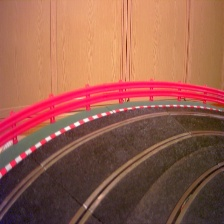
\includegraphics[width=4cm]{figs/imagedataset}\hspace{1cm}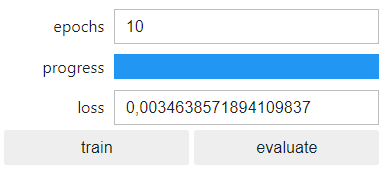
\includegraphics[width=6cm]{figs/epoch}
	\end{center}
	\caption{Imagen del \textit{dataset} utilizado entrenado con luz artificial y error al finalizar el entrenamiento.}
	\label{fig:imagedataset}
\end{figure}\

Una vez probada la red neuronal \textit{YOLO V3 Tiny} utilizada en el entorno simulado, se comprobó que era necesario bajar demasiado el límite o \textit{threshold} de detección, hasta 0.3, para poder detectar los objetos elegidos. A diferencia del entorno de simulación ,en el que dicho límite se fijó a 0.8. Esto provocaba falsos positivos y por tanto una detección poco fiable. Dicha circunstancia puede ser debida, entre otros motivos, a unos objetos reales algo distintos respecto a los que la red fue entrenada o una luz ambiental baja. Por ello se decidió entrenar la red con los objetos utilizados en el entorno real. Para ello, es necesario una tarjeta gráfica potente. Por lo que se realizó una comparativa entre las tarjetas gráficas disponibles para realizar el entrenamiento en el menor tiempo posible. Dicha comparativa está representada en el Cuadro \ref{table:versusnvidia}.\\

\begin{table}[H]
	\begin{center}
		\begin{tabular}{|c|c|c|c|c|}
			\hline
			\textbf{Placa}	& \textbf{Arquitectura} & \textbf{C.C\makebox[0pt][l]{$^*$}} & \textbf{GPU Cores}				& \textbf{RAM}
			\\
			\hline
			NVIDIA Jetson Nano		& Maxwell								& 5.3														& 128												& 4 GB
			\\
			NVIDIA MX330					& Pascal								& 6.1														& 384												& 2 GB
			\\
			NVIDIA AGX Xavier			& Volta									& 7.2														& 384 con 48 Tensor Cores		& 64 GB
			\\
			\hline
		\end{tabular}
		\parbox[t]{\textwidth}{\footnotesize C.C$^*$: capacidad de cómputo.}  
		\caption{Comparación entre las tarjetas gráficas disponibles para entrenar la red \textit{YOLO V3 Tiny}.}
		\label{table:versusnvidia}
	\end{center}
\end{table}

\subsection{Entrenamiento de la red \textit{YOLO V3 Tiny} para detección de objetos propios}
El objetivo es entrenar la red \textit{YOLO V3 Tiny} con el objetivo de poder detectar objetos propios o mejorar la probabilidad de detección de objetos ya detectados por la red.\\

Para ello, es pertinente saber qué \textit{dataset} se ha utilizado para generar los pesos actualmente usados. Atendiendo a la página oficial de \textit{YOLO\footnote{\url{https://pjreddie.com/darknet/yolo/}}}, el \textit{dataset} utilizado es \textit{COCO}. Por lo que será necesario obtener las imágenes y sus ficheros de etiquetado donde se asocian los objetos presentes en las imágenes. Existe un repositorio\footnote{\url{https://github.com/KaranJagtiani/YOLO-Coco-Dataset-Custom-Classes-Extractor}} que permite la extracción, a partir del \textit{dataset} mencionado, de las clases de objetos deseadas.\\

El formato del archivo de etiquetado de los objetos es muy relevante. El formato por defecto de \textit{COCO} es el contenido en el Código \ref{cod:formatcoco}\footnote{\url{https://cocodataset.org/\#format-data}}. Y el utilizado en \textit{YOLO} es el contenido en el Código \ref{cod:formatyolo}\footnote{\url{https://github.com/AlexeyAB/darknet\#how-to-train-to-detect-your-custom-objects}}. Por lo que es necesario realizar la conversión de un formato a otro. Este proceso también lo realiza el programa contenido en el repositorio anteriormente mencionado.\\

\begin{code}[h]
	\begin{lstlisting}
		annotation{
			"id": int, 
			"image_id": int, 
			"category_id": int, 
			"segmentation": RLE or [polygon], 
			"area": float, 
			"bbox": [x,y,width,height], 
			"iscrowd": 0 or 1,
		}

		categories[{
			"id": int, 
			"name": str, 
			"supercategory": str,
		}]
	\end{lstlisting}
	\caption[Formato de etiquetado de objetos utilizado por \textit{COCO}.]{Formato de etiquetado de objetos utilizado por \textit{COCO}.}
	\label{cod:formatcoco}
\end{code}

\begin{code}[h]
	\begin{lstlisting}
		<object-class> <x_center> <y_center> <width> <height>
	\end{lstlisting}
	\caption[Formato de etiquetado de objetos utilizado por \textit{YOLO}.]{Formato de etiquetado de objetos utilizado por \textit{YOLO}.}
	\label{cod:formatyolo}
\end{code}

Como se mencionó en el Capítulo 2, se ha utilizado la librería \textit{LabelIMG} para realizar el etiquetado de los objetos y generar el archivo en formato compatible con \textit{YOLO}. En la Figura \ref{fig:customlabelimg} se representa el etiquetado de uno de los objetos reales con dicha librería.\\

\begin{figure} [h!]
	\begin{center}
		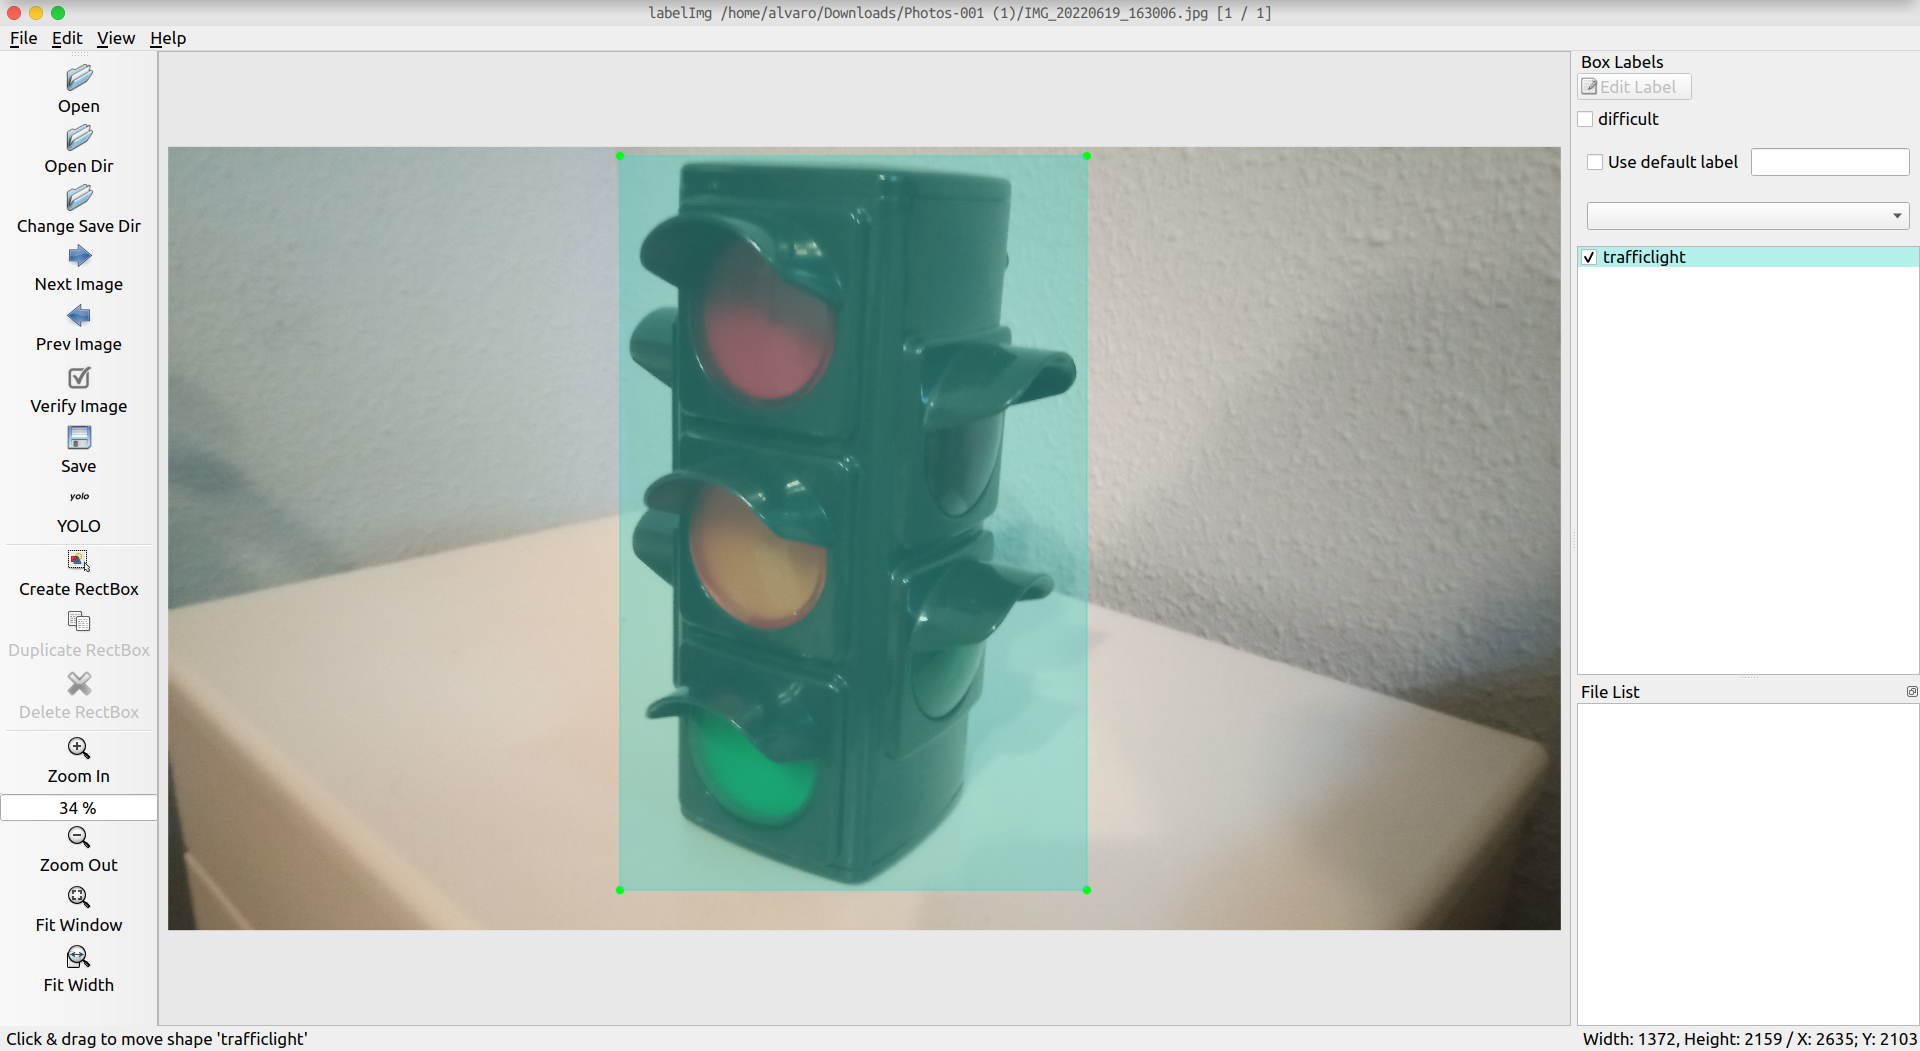
\includegraphics[width=12cm]{figs/customlabelimg}
	\end{center}
	\caption{Etiquetado de objetos propios con la herramienta \textit{LabelIMG}.}
	\label{fig:customlabelimg}
\end{figure}\

El gráfico representado en la Figura \ref{fig:graphcoco}, extraído de la siguiente fuente\cite{graphcoco}, muestra el número de imágenes de cada tipo de objeto. Se puede observar que el la clase persona está presente en imágenes, seis veces más que cualquier otro tipo de objeto. Esto se debe a que existen multitud de personas con distinto aspecto y por ello es necesario una cantidad muy grande de imágenes para obtener una detección fiable. Esto es determinante a la hora del entrenamiento, ya que al ser tan elevado el número de imágenes, el tiempo de entrenamiento será considerablemente grande.\\

\begin{figure} [h!]
	\begin{center}
		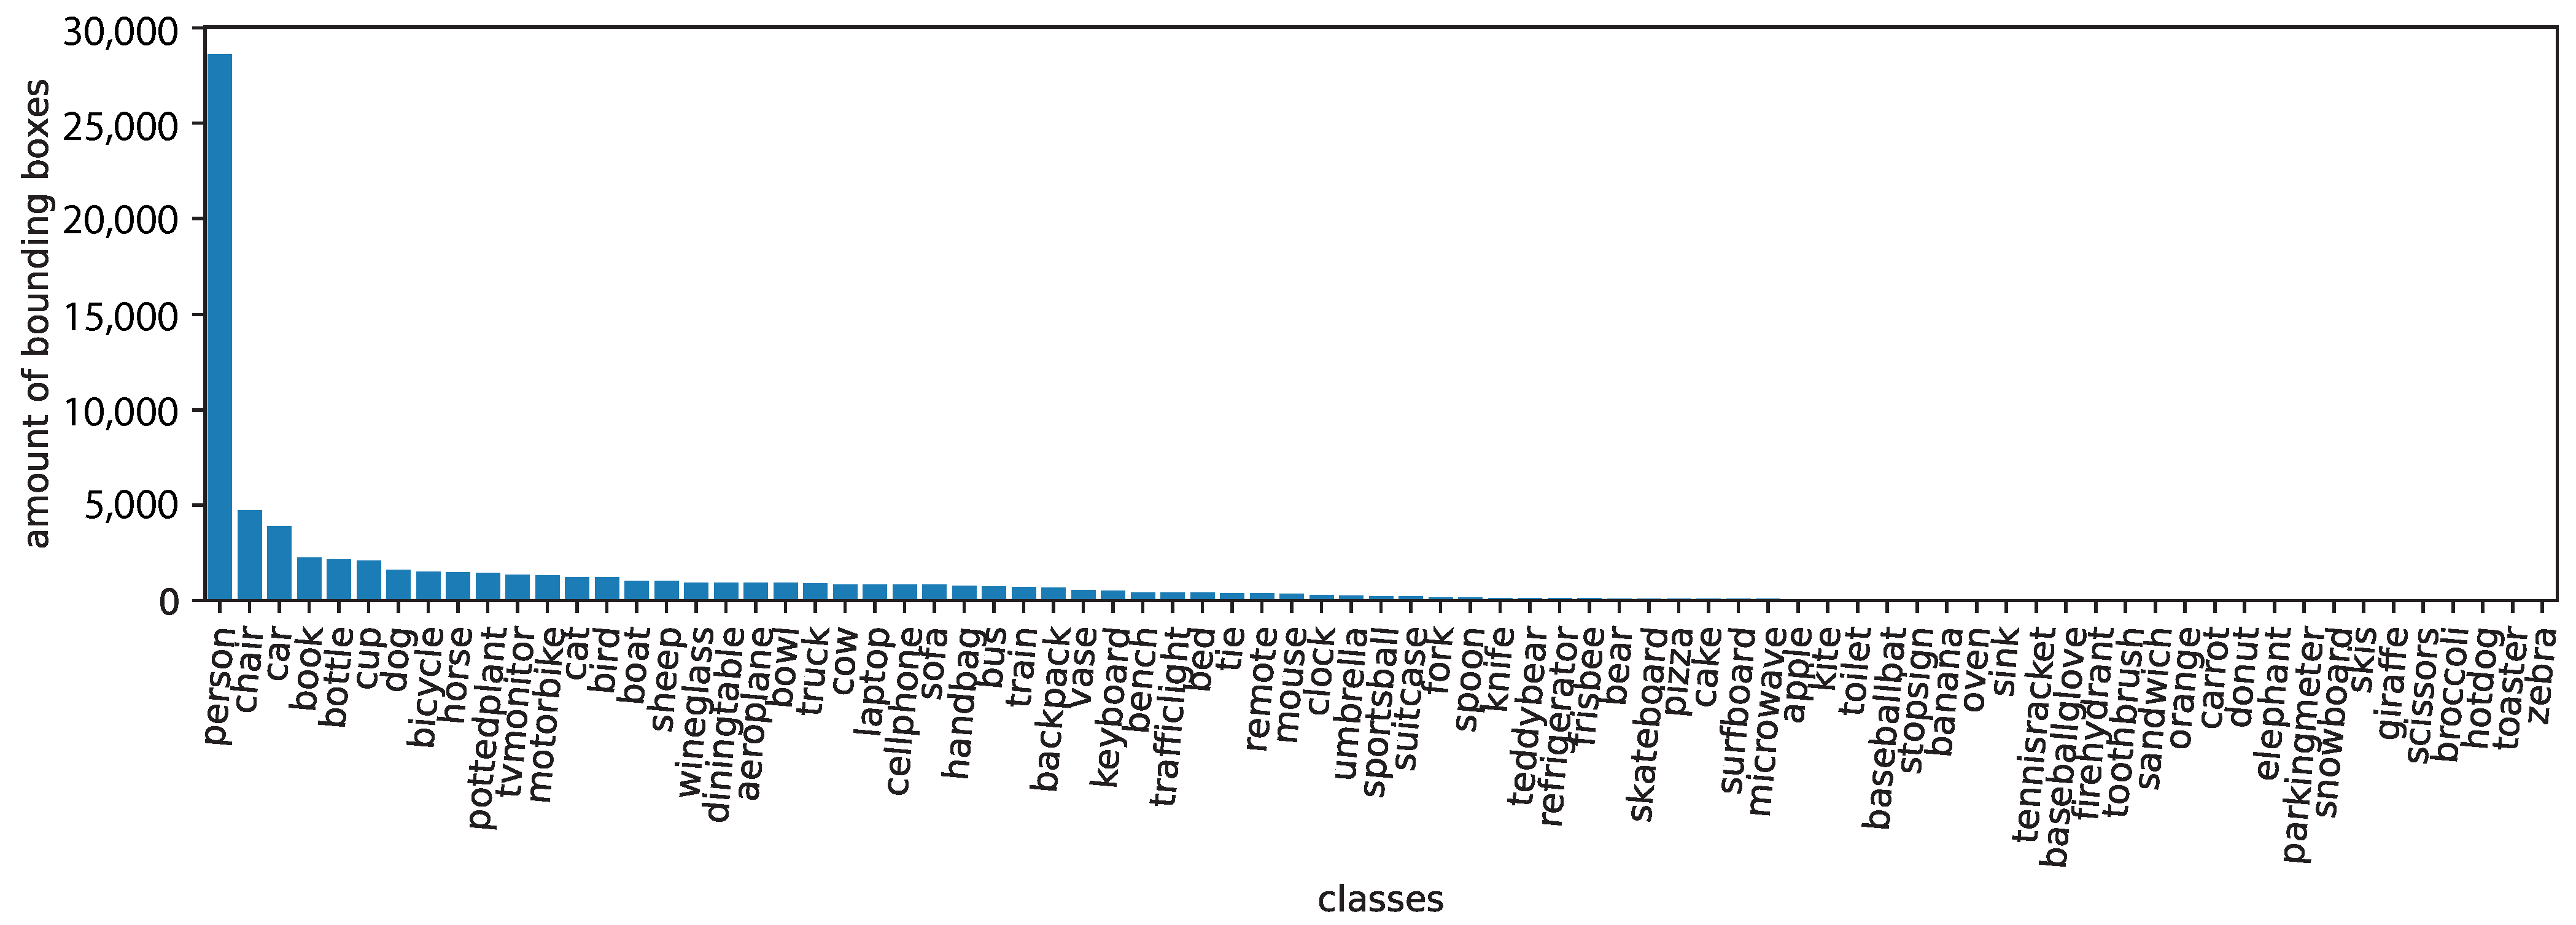
\includegraphics[width=14cm]{figs/graphcoco}
	\end{center}
	\caption{Distribución de las clases de objetos del \textit{dataset} COCO.}
	\label{fig:graphcoco}
\end{figure}\

Para proceder al entrenamiento, además del \textit{dataset} y sus ficheros de etiquetado, es necesario utilizar el \textit{framework} \textit{Darknet\footnote{\url{https://github.com/pjreddie/darknet}}} y hacer uso del comando \verb|partial| para obtener los pesos preentrenados sobre los cuales, se entrenará la red con el \textit{dataset} elegido.\\

También es necesario modificar una serie de archivos entre los que se encuentra el \textit{cfg} que contiene los parámetros de la red. Las principales modificaciones a realizar son las siguientes:
\begin{itemize}
	\item El número de \textit{batch} deberá ser 64.
	\item El número de \textit{subdivisions} deberá ser 2.
	\item El número de \textit{max\_batches} deberá ser el número de clases multiplicado por 2000. Y este número no debe ser inferior al número total de imágenes.
	\item El número de \textit{steps} deberá ser fijado al 80\% y al 90\% de \textit{max\_batches}.
	\item La anchura y altura de la imagen con la que entrena la red deberá ser como mínimo 416. En el caso de querer detectar objetos muy pequeños dicho parámetro deberá ser modificado a 608 o 832.
	\item En cada parámetro \textit{[yolo]} el número de clases de objetos a detectar deberá ser fijado y el número de \textit{filters} deberá fijarse atendiendo a la siguiente fórmula: \textit{(classes + 5) x 3}.
\end{itemize}\

Se deberán crear los ficheros \textit{train.txt} y \textit{test.txt} donde deben estar las rutas absolutas a cada fichero de etiquetado. Y otro fichero llamado \textit{obj.data} que contenga las rutas de los archivos anteriormente descritos, dicho contenido está presente en el Código \ref{cod:objdata}.\\

\begin{code}[h]
	\begin{lstlisting}
		classes = 9
		train  = data/train.txt
		valid  = data/test.txt
		names = data/obj.names
		backup = backup/
	\end{lstlisting}
	\caption[Contenido del archivo \textit{obj.data} con las rutas de los archivos necesarios.]{Contenido del archivo \textit{obj.data} con las rutas de los archivos necesarios.}
	\label{cod:objdata}
\end{code}

Otro factor importante es el porcentaje de imágenes con el que no se entrena la red pero sí prueba para comprobar la validez de la misma. Estas imágenes componen el \textit{dataset} de validación y debe estar compuesto por un 20\% de las imágenes totales del \textit{dataset}.\\

Durante el entrenamiento se irá mostrando una gráfica que indica el progreso, representada en la Figura \ref{fig:chart}. En dicha gráfica se muestra el error de la red, se puede observar que el error final tras terminar el entrenamiento es de 0.663. Atendiendo a la guía\footnote{\url{https://github.com/AlexeyAB/darknet\#how-to-train-to-detect-your-custom-objects}} utilizada para entrenar la red, el error deberá estar entre 0.05 en el caso de un \textit{dataset} pequeño y simple a 3.0 en el caso de un \textit{dataset} grande y difícil, como es el caso de la clase persona.\\

\begin{figure} [h!]
	\begin{center}
		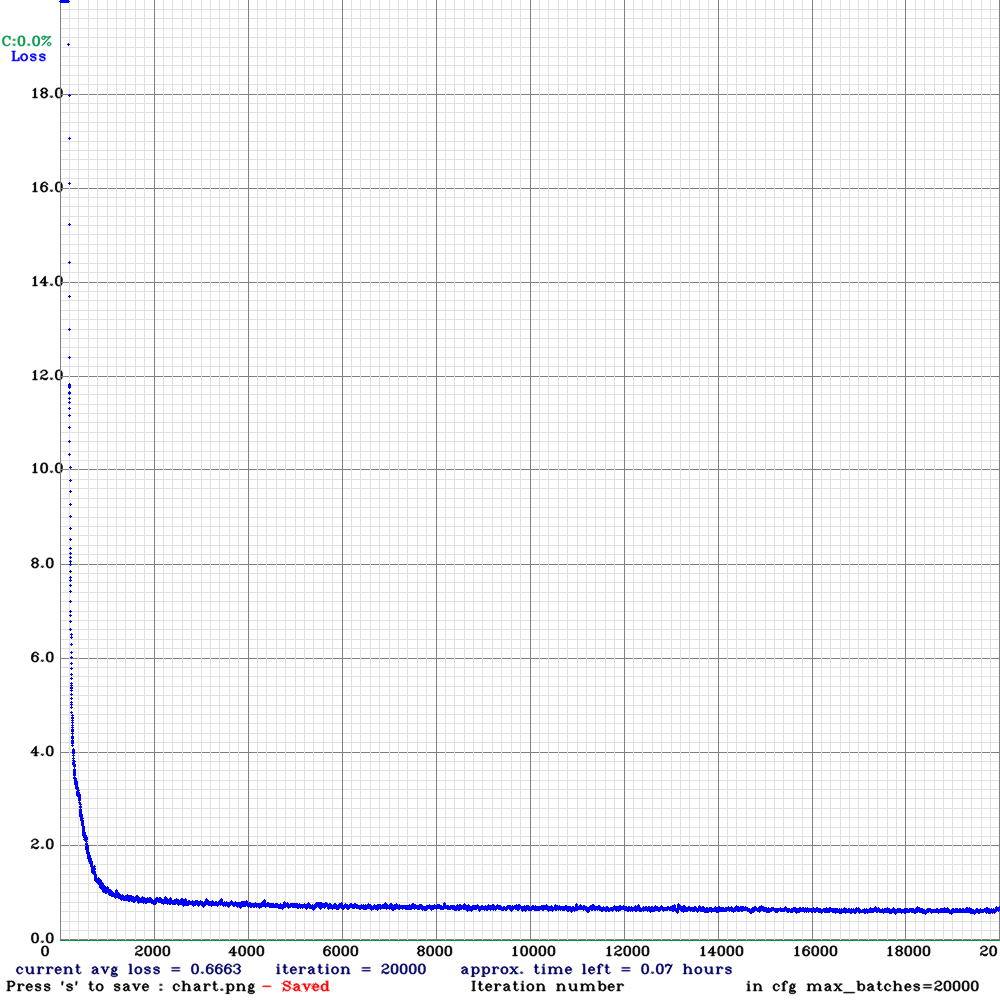
\includegraphics[width=12cm]{figs/chart}
	\end{center}
	\caption{Gráfica de entrenamiento mostrando el error de la red \textit{YOLO V3 Tiny}.}
	\label{fig:chart}
\end{figure}\

\subsection{Controlador diseñado para el seguimiento de carril a partir de la salida de la red neuronal}
Una vez obtenida la salida de la red neuronal que indica el centro del carril, es necesario elaborar un controlador que comande velocidades lineales y angulares al robot. Para ello se ha realizado un controlador proporcional (P) con una serie de constantes para lograr un comportamiento adecuado, dicho controlador está disponible en el Código \ref{cod:controller}.\\ 

\begin{code}[h]
	\begin{lstlisting}[language=Python]
		def setSteering(self, steering):
			if steering > self.FORWARD_RANGE:
				rightSpeed = self.STEERING_OFFSET + abs(steering * self.STEERING_GAIN)
				if rightSpeed < self.MIN_SPEED:
					rightSpeed = self.MIN_SPEED
				leftSpeed = self.TURNING_SPEED
				self.goRight()
			elif steering < -self.FORWARD_RANGE:
				leftSpeed = self.STEERING_OFFSET + abs(steering * self.STEERING_GAIN)
				if leftSpeed < self.MIN_SPEED:
					leftSpeed = self.MIN_SPEED
				rightSpeed = self.TURNING_SPEED
				self.goLeft()
			else:
				self.goForward()
				leftSpeed = self.throttleMotor
				rightSpeed = self.throttleMotor
			
			self.setSpeed(leftSpeed, rightSpeed)
	\end{lstlisting}
	\caption[Controlador P realizado para el seguimiento de carril.]{Controlador P realizado para el seguimiento de carril.}
	\label{cod:controller}
\end{code}

\subsection{Transformación del modelo de \textit{PyTorch a TensorRT}}
Como se expuso en el Capítulo 3, existe una librería llamada \textit{PyTorch to TensorRT} capaz de convertir modelos de \textit{PyTorch} a modelos optimizados aprovechando los tensores de las gráficas dedicadas, si bien la placa \textit{NVIDIA Jetson Nano} no dispone de una GPU con tensores\footnote{\url{https://connecttech.com/jetson/jetson-module-comparison/}}, sí permite realizar inferencia utilizando operaciones con \textit{FP16} lo que aumenta el rendimiento en gran medida. Esta conversión se realiza de forma muy sencilla llamando a la función \verb|torch2trt()| tal y como representa el Código \ref{cod:torch2trt}.\\

\begin{code}[h]
	\begin{lstlisting}[language=Python]
		data = torch.zeros((1, 3, 224, 224)).cuda().half()
		model_trt = torch2trt(model, [data], fp16_mode=True)
		torch.save(model_trt.state_dict(), 'model_tensor.pth')
	\end{lstlisting}
	\caption[Conversión del modelo para realizar optimización y aumentar el rendimiento.]{Conversión del modelo para realizar optimización y aumentar el rendimiento.}
	\label{cod:torch2trt}
\end{code}

En la Figura \ref{fig:screenshotsreal} están representadas capturas de la ejecución en el entorno real desde la perspectiva de la visión del robot.\\

\begin{figure} [h!]
	\begin{center}
		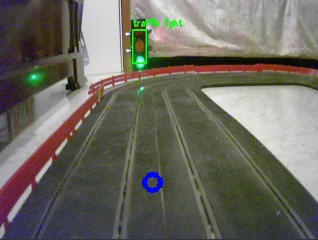
\includegraphics[width=6cm]{figs/screenshottrafficlight}\hspace{0.5cm}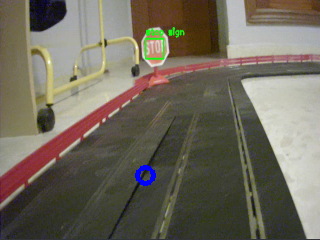
\includegraphics[width=6cm]{figs/screenshotstopsign}
	\end{center}
	\caption{Visión del robot durante la ejecución en el entorno real.}
	\label{fig:screenshotsreal}
\end{figure}\

\section{Diseño del software a partir de un diagrama de clases}
El diseño del software se ha realizado a partir de un diagrama de clases, utilizando la herramienta \textit{UMLET\footnote{\url{hhttps://www.umlet.com/}}}, que permite estructurar crear clases, dependencias entre ellas y los atributos y funciones que contiene. El presente diseño, representado en la Figura \ref{fig:diagram}, contiene una clase principal llamada \textit{AutonomousVehicle} que tiene instancias de la clase \textit{LaneFollower} que implementa el seguimiento de carril, de la clase \textit{JetRacer} que implementa el controlador del vehículo y la comunicación con los motores del mismo. También contiene una instancia de la clase \textit{ObjectDetector} que implementa la detección de objetos y, a su vez, la clase \textit{ObjectDetector} hace uso del flujo de vídeo proveniente de un \textit{topic} de \textit{ROS}.
\begin{figure} [h!]
	\begin{center}
		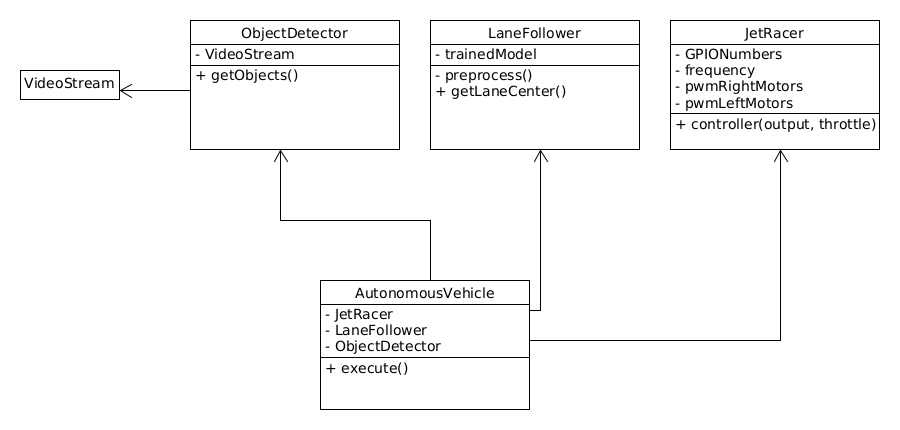
\includegraphics[width=14cm]{figs/diagram5}
	\end{center}
	\caption{Diagrama de clases.}
	\label{fig:diagram}
\end{figure}\
% Tabla cámara
% Buscar ....
% Gráfica entrenamiento error no sube ni baja, estable carril
% Resnet
% NN siempre yxy?
% .yaml stop or stop sign?
% Tesnor cores
% yolov3-tiny.conv.15 15 convolución 15
% singlestone
% \textit{Over-fitting}
% muestra el número de imágenes??????? y causas
% Salir de sección screenshotsreal
% screenshot red hsv traffic light
